\documentclass[]{usiinfbachelorproject}

\usepackage{todonotes}
\usepackage{soul}
\usepackage{dirtytalk}
\usepackage{subcaption}
\usepackage[nottoc]{tocbibind}

\captionsetup{labelfont={bf}}
%\setlength{\parindent}{0cm}

\author{Davide Ciulla}

\title{Stack and Heap Diagrams}
\subtitle{A Graphical Editor}
\versiondate{\today}

\begin{committee}
%With more than 1 advisor an error is raised...: only 1 advisor is allowed!
\advisor[Universit\`a della Svizzera Italiana, Switzerland]{Prof.}{Matthias}{Hauswirth}
%You can comment out  these lines if you don't have any assistant
%\assistant[Universit\`a della Svizzera Italiana, Switzerland]{Title}{AssistantName1}{AssistanSurname1}
%\assistant[Universit\`a della Svizzera Italiana, Switzerland]{Title}{AssistantName2}{AssistanSurname2}
\end{committee}

\abstract{
Teaching students the fundamentals of programming is not an easy task at all, but luckily there are useful tools like stack and heap diagrams that can facilitate this process, by providing professors ways to easily assess the students understanding on a given topic. However, these diagrams are often drawn either on paper or with legacy software that must be installed on the computer. In this project, I developed a web-based stack and heap graphical editor, using modern front-end web technologies like React and Sass.}



\begin{document}

\maketitle


\tableofcontents
\newpage


%%%%%%%%%%%%%%%%%%%%%%%%%
\section{Introduction} \label{introduction}
%%%%%%%%%%%%%%%%%%%%%%%%%

In this first section I am going to describe all the thoughts that went into this project at the very early stages, from the moment I first discussed the project with prof. Hauswirth, to the moment right before starting the pre-production phase (see \hyperref[requirements+analysis]{\textbf{Section 3}}).

\subsection{Theoretical background}

\noindent In the world of computer science, stack and heap are two very important memory allocation areas. The stack is a LIFO (\emph{Last In First Out}) data structure responsible for keeping track of function calls. Every time a function is called, a new stack frame is pushed onto the stack, containing its parameters, its local variables
 and the return address\footnote{\url{https://medium.com/fhinkel/confused-about-stack-and-heap-2cf3e6adb771}}. Stack frames only exist during the execution of a function, and are popped from the stack when the latter has completed its lifecycle.\\
 Conversely, the heap does not have a LIFO structure and it is independent from the program execution, being a segment of memory dedicated to dynamic memory allocation. When we program and allocate memory, we create objects on the heap. In some programming languages (like C and C++), these objects do not disappear automatically and they must be manually deallocated by the programmer (bad heap management can cause memory leaks - a failure in a program to release discarded memory, causing impaired performance or failure\footnote {\url{https://en.wikipedia.org/wiki/Memory_leak}}).\\
 
\begin{figure}[h!]
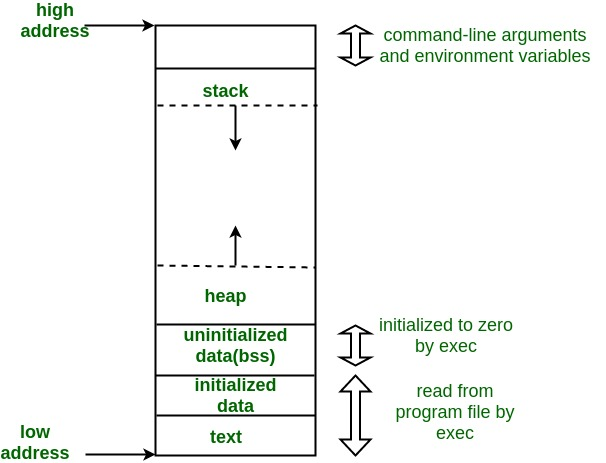
\includegraphics[scale=0.4]{figures/memory_layout.jpg}
\centering
\caption {Generalized memory layout of a program}
\end{figure}
 
\noindent Another important concept to clarify is the notional machine. It was first introduced by \emph{Benedict du Boulay} in 1986 with the article \emph{Some Difficulties of Learning to Program} \cite{boulay}, and it can be described as a set of abstractions that define the structure and behavior of a computational device \cite{guzdial_et_al:DR:2019:11627}. The goal of such a machine is not to be an exact replica of the real device, because by providing abstractions it is hopefully easier for students to understand the real machine \cite{7743153}. Students build their mental models about the notional machine through teaching, learning methods and materials used in programming classes \cite{HIDALGO-CESPEDES2016}.\\
My web application is an example of a such a machine.
 
\begin{figure}[h!]
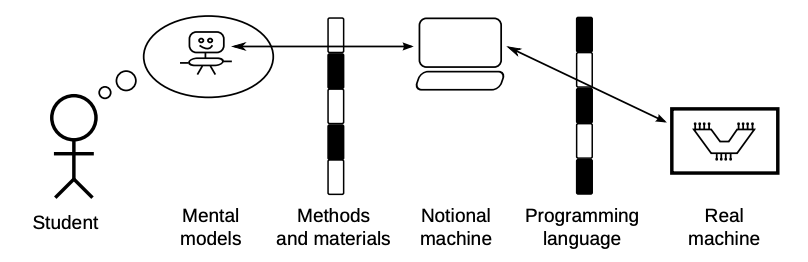
\includegraphics[scale=0.8]{figures/notional_machine.png}
\centering
\caption {Process of creating mental models about notional machines}
\end{figure}
 
\vspace{\fill}
\pagebreak
 
\noindent Finally, I also want to explain what clicker tools are, since my work was based on recreating and improving a subset of features implemented in the Informa clicker (see \hyperref[informa clicker]{\textbf{Section 2.1}}). According to the Luce Group\footnote{\url{http://luce.inf.usi.ch/}}, ``a clicker is a special purpose remote control used in traditional group response systems, where an instructor projects a multiple-choice question on the classroom projector and students use these tools to submit their answers by pressing one of the buttons. The advantage of using such systems is that the instructor has immediate feedback on the students understanding, by seeing their responses aggregated in the form of a histogram.'' \footnote{\url{http://sape.inf.usi.ch/informa}}
 
\subsection{Motivation}

As I am going to show in \hyperref[state]{\textbf{Section 2}} about state-of-the-art projects for programs visualizations, one can do a quick Google search and see that there are already tools in the real world that help students grasp important computer science topics, by showing the state of their code at each point of its execution.\\
However, the majority of them are automated, meaning that they take real code as input and automatically create diagrams as outputs. With such programs, \textbf{students cannot demonstrate their understanding}, and \emph{that} is exactly why I am making this application.

\subsection{Goal} \label{goal}

The goal of this project is to create a web application inspired by the Informa clicker tool, that allows students to very easily create stack and heap diagrams to visualize the structure of their code and better understand what is actually happening under the hood. This kind of diagram can give very useful insights both to the student and to the professor.\\ This application is planned to be integrated into Informa (prof. Hauswirth's web platform for his Programming Fundamentals 2 course), but it can also be used as a standalone application. That way, students can not only use it in class during class exercises, but also for instance at home while studying on their own.\\
Furthermore, a JavaScript object containing the data representation of the diagram is constantly kept up-to-date with every state change happening, which can be used for automatic testing and potentially instant feedback on the correctness of their diagrams.

\subsection{Use cases}

This application was developed with the two following use cases in mind:

\begin{enumerate}
\item Teacher provides some code and an arbitrary breakpoint, and the student must create  a diagram mirroring the state of the program when the breakpoint is reached.
\item Teacher draws a diagram and student must be able to describe the current state of the program execution.
\end{enumerate}

\vspace{\fill}
\pagebreak

%%%%%%%%%%%%%%%%%%%%%%%%%
\section{State of the Art} \label{state}
%%%%%%%%%%%%%%%%%%%%%%%%%

In this section I am going to showcase projects that I consider to be state-of-the-art in terms of visual representations of code. Not all of them are related to stack and heap diagrams, but they do still set a benchmark for graphical output and ease of learning.

\subsection{Informa Clicker - Luce Group} \label{informa clicker}

\noindent Informa \footnote{\url{https://informa.inf.usi.ch/}} is not only a teaching platform, but it also has a clicker tool available for download, that students can use to solve interactive problems. One of the problems they can solve is showing the correct state of a stack and heap diagram at a given point of a code execution.

\noindent In the diagram, users can create moveable stack frames (grey rectangles) and objects (red rectangles) on the heap. Stack frames and objects have different labels (method signature for stack frames and class name for objects), but they both can store primitive and reference variables. All variables have fields for writing the variable name, type and value. In case of reference variables, the value is the reference to another object, which is represented by an arrow.\\

\noindent This clicker tool was developed by professor Matthias Hauswirth, my bachelor thesis advisor, for the Luce Group.

\begin{figure}[h!]
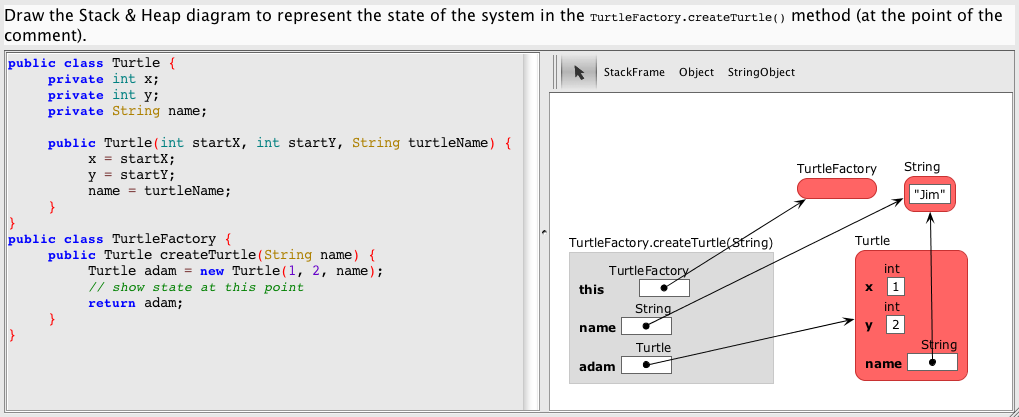
\includegraphics[scale=0.4]{figures/informa_clicker.png}
\centering
\caption {Stack and heap diagrams in the Informa clicker tool}
\end{figure}

\subsection{BlueJ - King's College London}

BlueJ \footnote{\url{https://www.bluej.org/}} (see \hyperref[bluej_classes_objects]{\textbf{Figure 4}} and \hyperref[bluej_objects_open]{\textbf{Figure 5}}) is free Java IDE (\emph{Integrated Development Environment}) designed for beginners, developed by the King's College London and officially supported by Oracle, the company that owns the Java platform.
The aspect that makes BlueJ stand out from the other IDEs is its powerful main view, which shows an interactive diagram of the different elements that compose your source code. It also renders arrows that are very useful, because they show how the different classes are interconnected. Objects are shown too, but they do not present any arrow.\\
BlueJ is also used in the textbook \emph{Objects First with Java: A Practical Introduction using BlueJ} by David J. Barnes \& Michael K\"{o}lling \cite{barnes2016objects}, a popular choice for programming fundamentals classes that use Java as the first step into the world of object oriented programming languages.

\begin{figure}[h!]
\centering
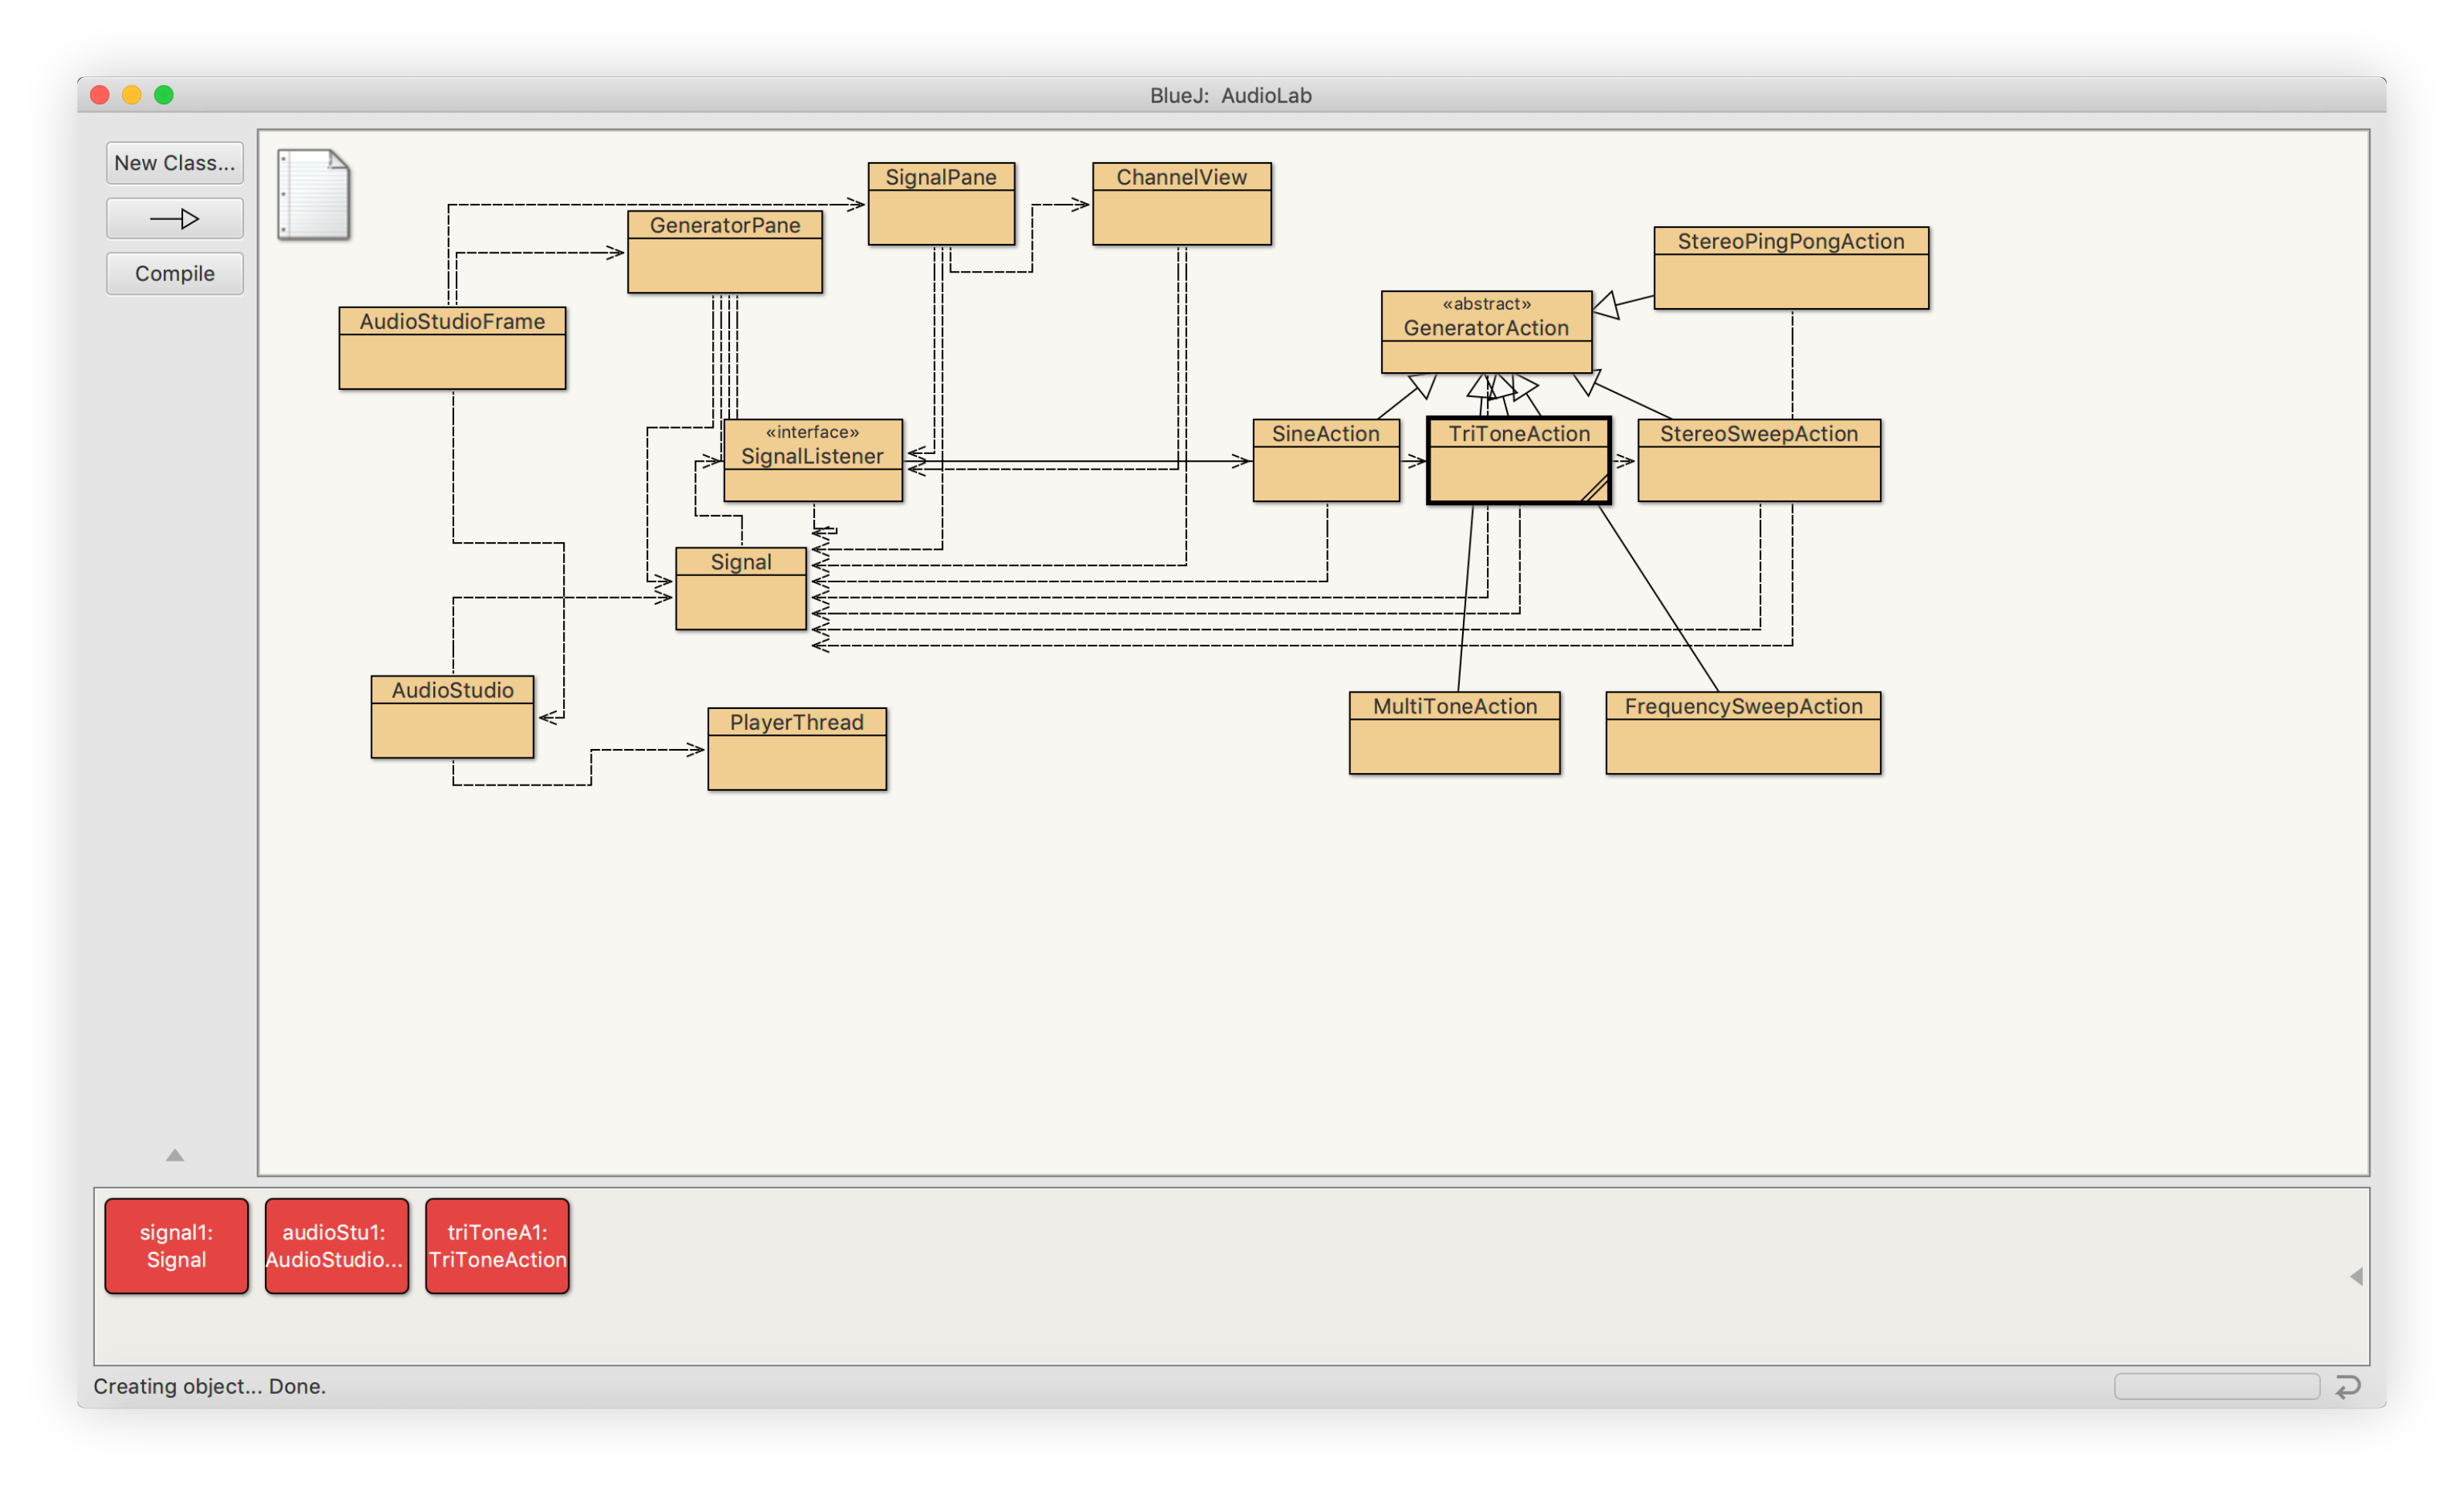
\includegraphics[width=\textwidth]{figures/bluej_classes_objects.png}
\caption {Main view of BlueJ showing classes and the arrows connecting them. On the bottom there is the Object Bench containing all the current class instances}
\label {bluej_classes_objects}
\end{figure}

\begin{figure}[h!]
\centering
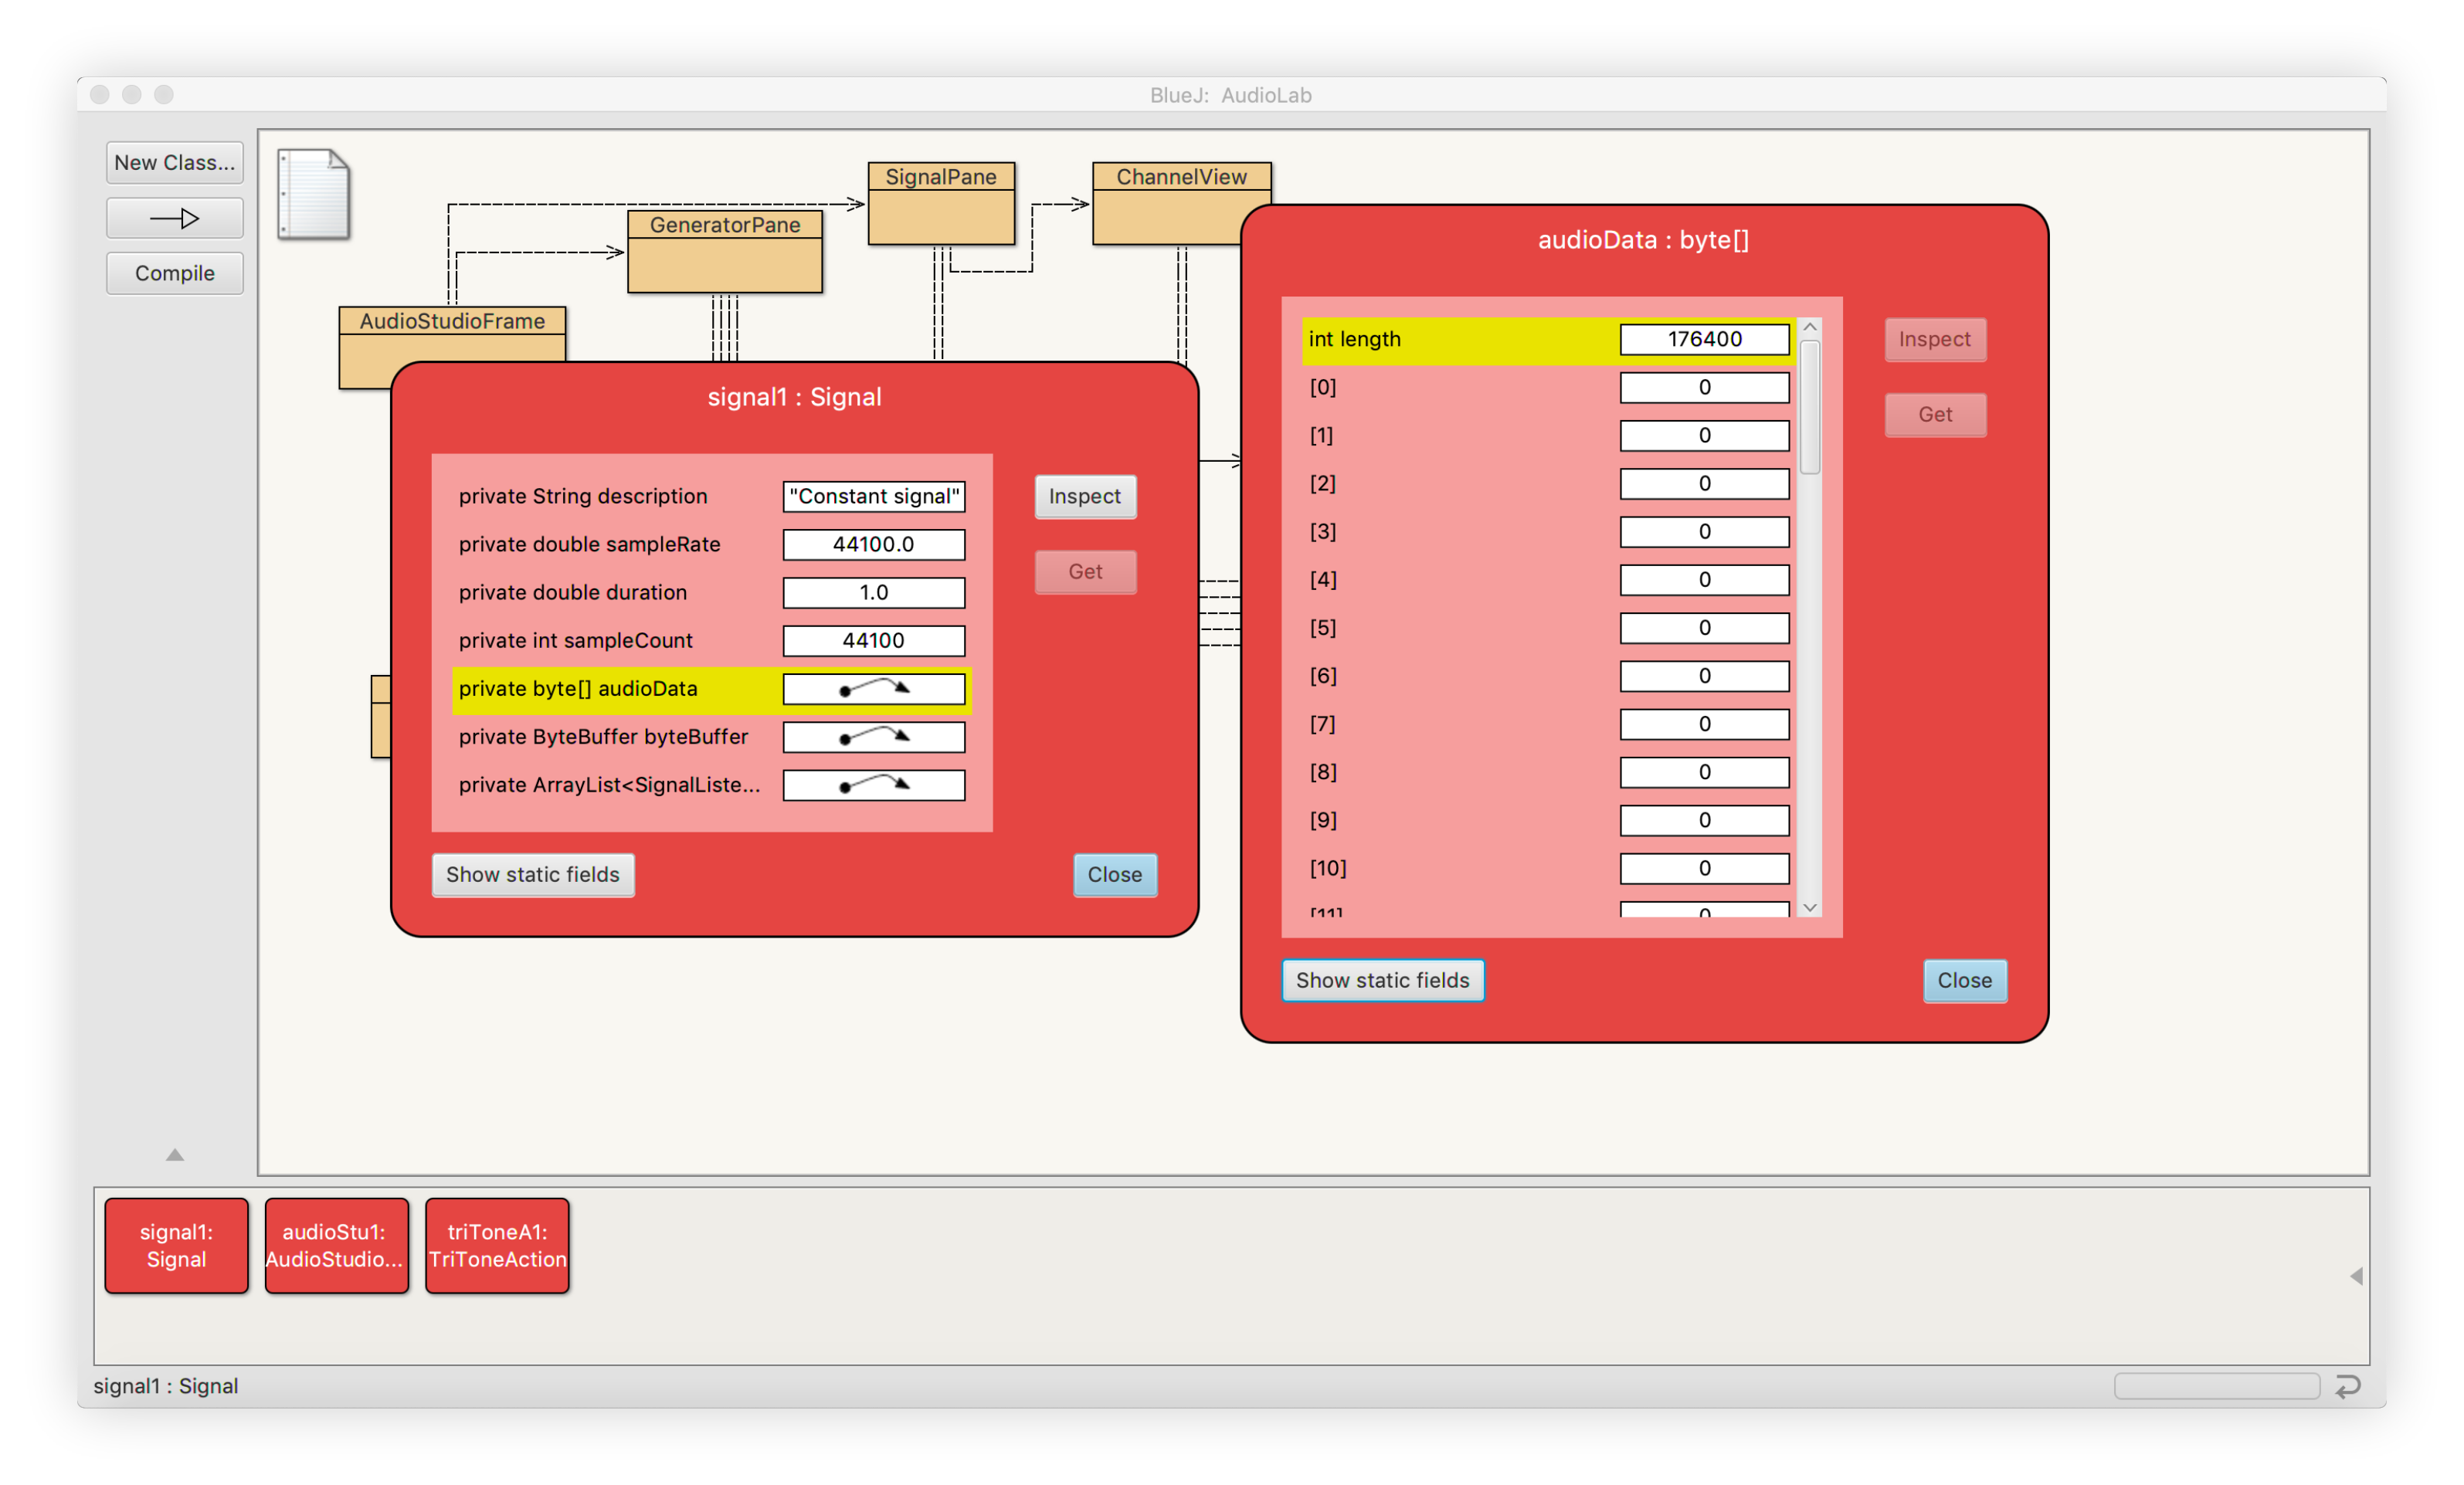
\includegraphics[width=\textwidth]{figures/bluej_objects_open.png}
\caption {Detailed view of an object in BlueJ. As you can see, arrows are only displayed in the main view and for classes. In the object view, reference variables have an arrow icon, which can be double clicked to see what they are referring to}
\label {bluej_objects_open}
\end{figure}

\subsection{Novis - Michael Berry \& Michael K\"{o}lling}

Novis \cite{7743153} is a notional machine implementation, aimed at beginners and integrated into BlueJ, providing real-time visualisation of the notional machine.

\begin{figure}[h!]
\centering
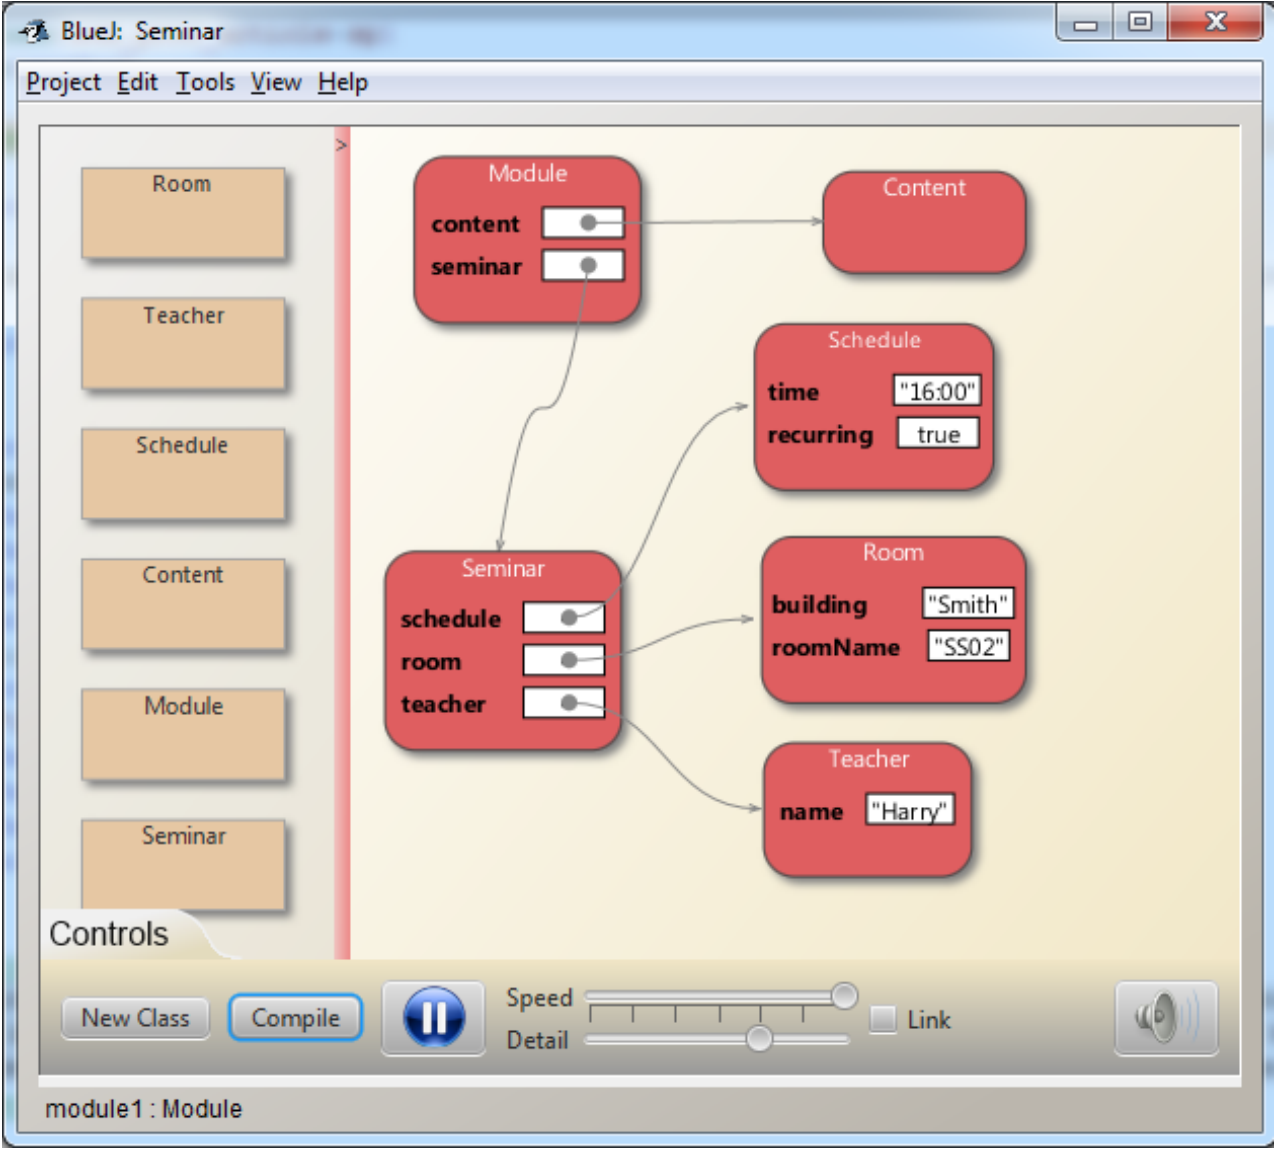
\includegraphics[scale=0.4]{figures/Novis.png}
\caption {Novis}
\end{figure}

\vspace{\fill}
\pagebreak

\subsection{JIVE - University at Buffalo, USA}

JIVE \footnote{\url{https://cse.buffalo.edu/jive/}} stands for \emph{Java Interactive Visualization Environment} and it is an interactive execution for the Eclipse IDE \footnote{\url{https://www.eclipse.org/}} that provides visualizations of Java programs. In particular, it features an object diagram that allows users to see the current objects on the heap and their interconnections using arrows.

\begin{figure}[h!]
\centering
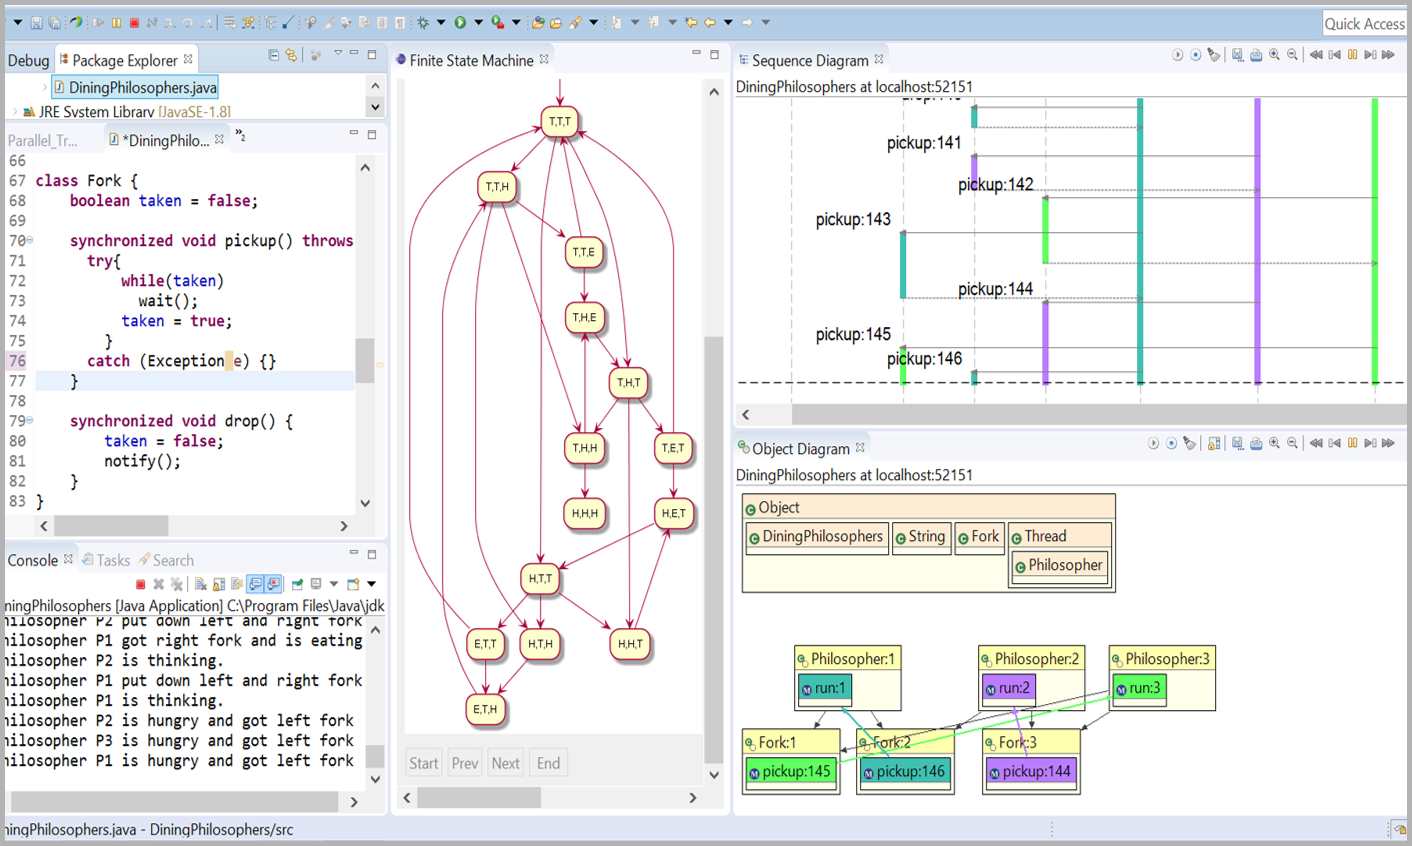
\includegraphics[width=\textwidth]{figures/jive.png}
\caption {JIVE}
\end{figure}

\subsection{ViLLE - University of Turku, Finland}

ViLLE \footnote{\url{https://ville.cs.utu.fi/old/}} is a multi-language program visualization tool developed by the University of Turku in Finland. Like other visualizers, its goal is to support the learning experience of beginner programmers, who might struggle to understand how to code. It has different use cases, for example it can be used to create and edit code snippets and to see in real time what happens during their execution.

\begin{figure}[h!]
\centering
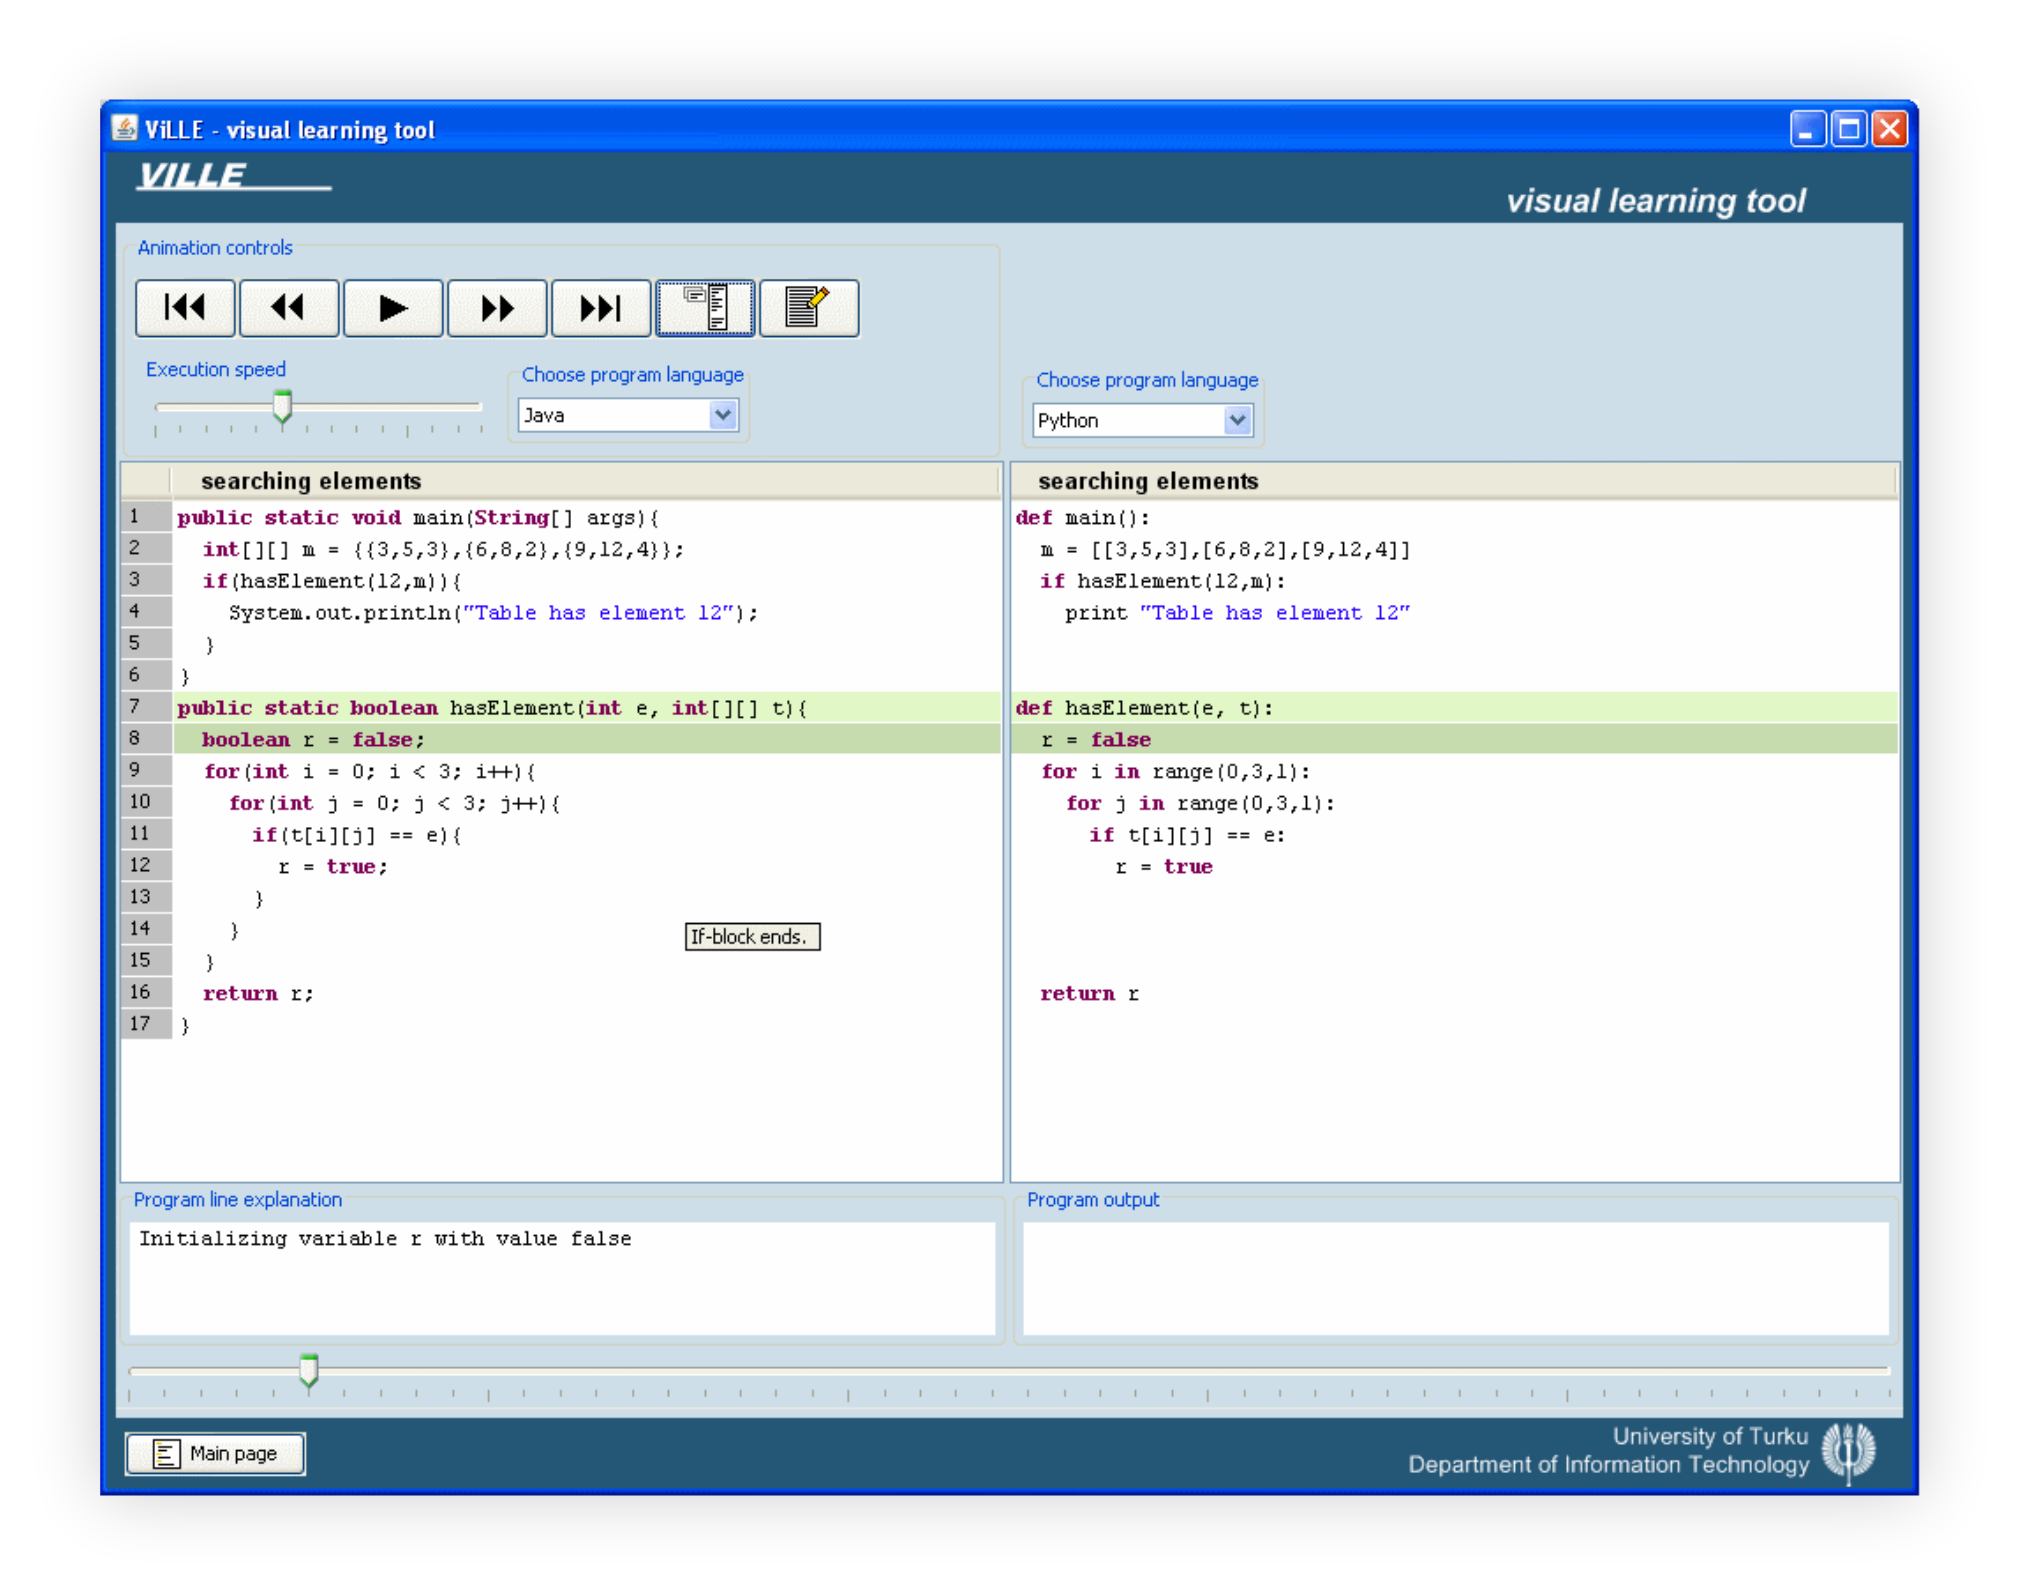
\includegraphics[scale=0.165]{figures/ville.png}
\caption {ViLLE}
\end{figure}

\subsection{Python Tutor}

Python Tutor \footnote{\url{http://www.pythontutor.com/}} is a web application for writing some code, see it visualized and executing step by step, and get live help from other users currently on the website.

\begin{figure}[h!]
\centering
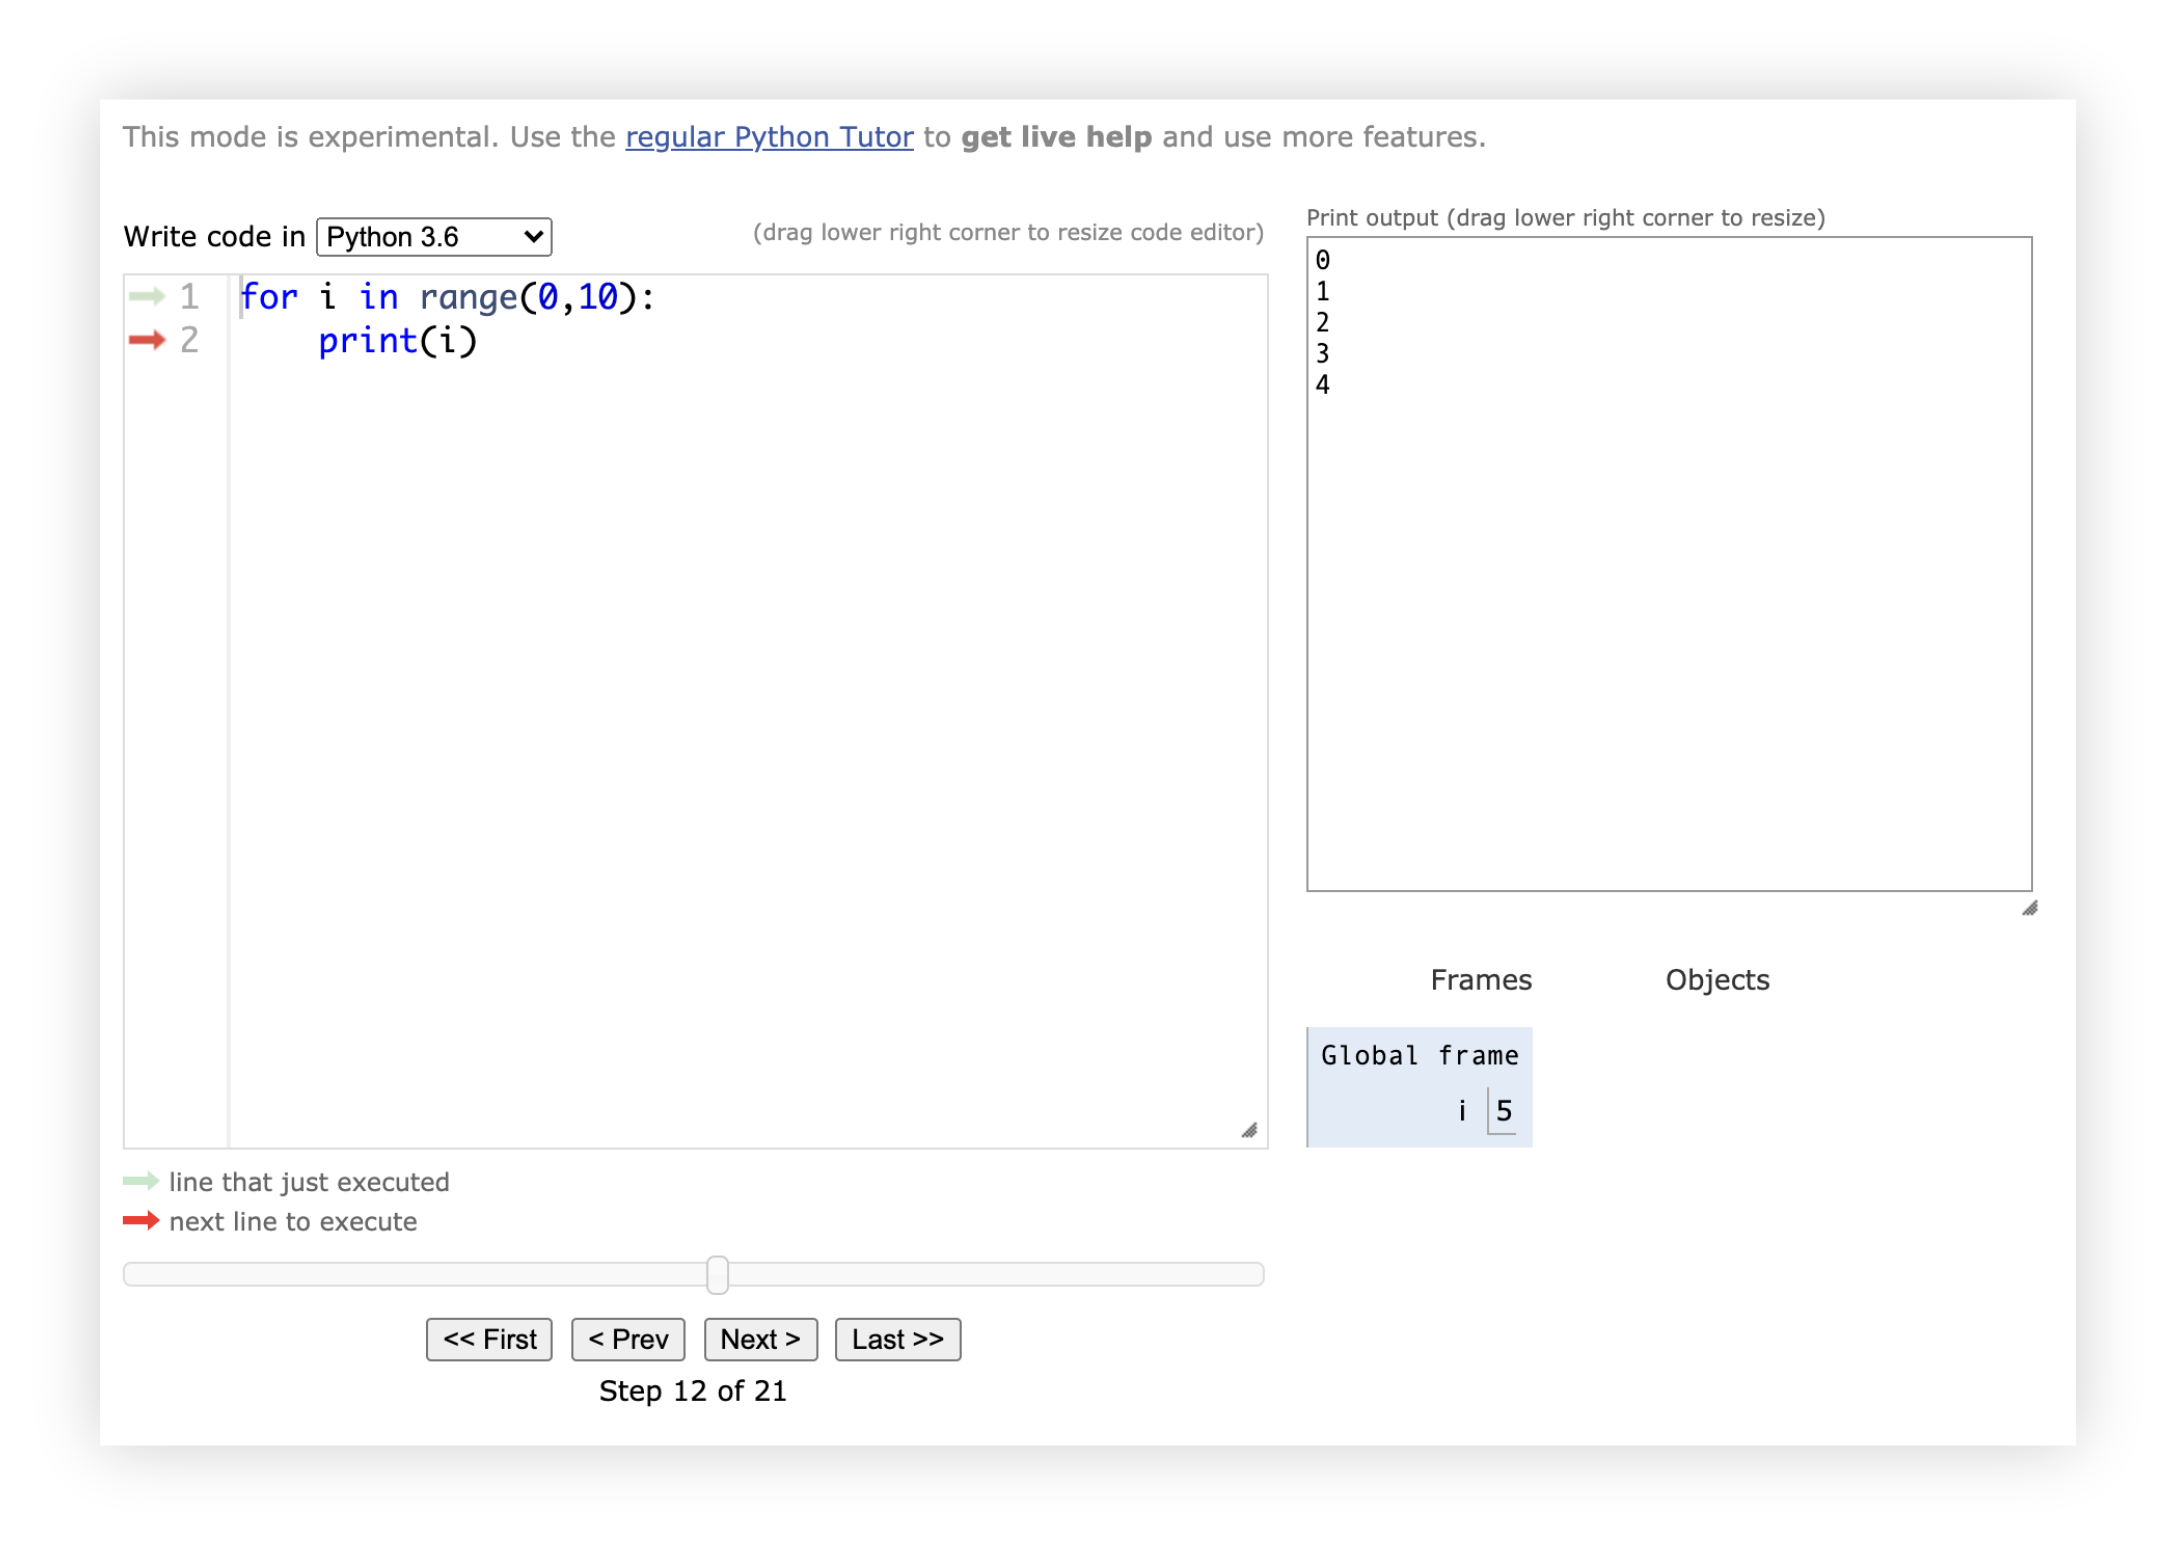
\includegraphics[scale=0.168]{figures/python_tutor}
\caption {Python tutor}
\end{figure}

\vspace{\fill}
\pagebreak

%%%%%%%%%%%%%%%%%%%%%%%%%
\section{Project analysis and requirements} \label{requirements+analysis}
%%%%%%%%%%%%%%%%%%%%%%%%%

In this section I am going to talk about the pre-production phase of the project, from the UI/UX analysis of the main Informa clicker tool, to the basic requirements that were decided as a baseline for the project.

\subsection{UI/UX analysis}

As already mentioned in \hyperref[goal]{\textbf{Section 1.3}}, the main goal of this project was to create an improved and web-based version of the already existing stack and heap diagram in the Informa clicker tool. In order to understand what worked and what did not work, I did an analysis of its user interface (UI) and user experience (UX) and here is what I found:\\

\textbf{\ul{UI - What works:}}

\begin{itemize}
	\item Arrows always point to the center of the target block, avoiding arrows overlapping.
	\item The interface has a good layout, as all elements are properly positioned following a clear and organized structure.
\end{itemize}\

\textbf{\ul{UI - What does not work:}}

\begin{itemize}
	\item Not enough overall white space \footnote{\url{https://blog.bannersnack.com/white-space-in-graphic-design/}}.
	\item Colors can be improved, because they do not convey a lot of excitement by being very pale. In this case, saturation can help to create a more engaging experience.
	\item All buttons that appear on mouseover events substantially clutter the interface and hide too many elements.
	\item The space dedicated to the diagram is relatively small compared to the whole screen.
	\item The buttons in the top toolbar are not styled as buttons.
\end{itemize}\

\textbf{\ul{UX - What works:}}

\begin{itemize}
	\item The interface is generally very intuitive thanks to its already praised layout, and I did not have any issues pursuing any task.
\end{itemize}\

\textbf{\ul{UX - What does not work:}}

\begin{itemize}
	\item The buttons at the top of the diagram, by not looking like buttons, make their purpose unclear to the user.
	\item Dragging the start of an arrow starting from a stack frame, makes it snap back to the border of a given block instead of the center of a variable.
	\item There is no clear distinction between stack and heap, except for the background color of stack frames and objects.
\end{itemize}\

\noindent As you can read from this analysis, the result is pretty clear: the Informa clicker does not have big problems in terms of user experience, but it lacks a proper user interface to better deliver what already works.

\vspace{\fill}
\pagebreak

\subsection{Requirements}

After running the UI/UX analysis and establishing that what had to be improved was the UI, prof. Hauswirth and I set as minimum requirements all the features the clicker already had. In particular users should have been able:

\begin{enumerate}
	\item Freely create stack frames and heap objects by dragging and dropping them onto the interface.
	\item Add and remove primitive and reference/instance variables from a given block \footnote{A block is a general term for stack frames and heap objects.}.
	\item Create arrows by clicking on a reference variable, holding that click and releasing it on a heap object.
	\item Drag blocks around.
\end{enumerate}

\noindent Plus something new:

\begin{enumerate}
	\item A data structure must be updated with every state change within the diagram (more on this is \hyperref[storing states]{\textbf{Section 4.4}}), and eventually be converted to a JSON file for offline editing and automated tests on Informa.
	\item Clear division between stack and heap.
\end{enumerate}

\subsection{Extra features}

Alongside the requirements, we have also agreed upon a set of possible bonus features that could be added if I would have finished the project early:

\begin{enumerate}
	\item The JSON file which represents the current state of the diagram, can both be downloaded and uploaded into the web application. Uploading that file acts like loading a save state in a videogame, because the whole interface goes back as it was left at the time of downloading the JSON file.
	\item Panning and zooming around in the interface.
	\item Arrows as polygonal chains \footnote{\url{https://en.wikipedia.org/wiki/Polygonal_chain}}.
\end{enumerate}

\vspace{\fill}
\pagebreak

%%%%%%%%%%%%%%%%%%%%%%%%%
\section{Project design} \label{design}
%%%%%%%%%%%%%%%%%%%%%%%%%

In this section I am going to describe the design process, not only coding-wise but also from the graphics perspective, elaborating all the decisions and solutions I had to make during this critical development phase. The design process can, in fact, either make or break the entire project. Making awful decisions at this stage, causes unavoidable problems down the line and it is the precise reason why I took maybe a bit more time than what I had initially planned, and only start coding when we were satisfied enough with the result.

\subsection{UI/UX research} \label{ui-ux research}

In \hyperref[requirements+analysis]{\textbf{Section 3}}, we saw how the biggest problem of the Informa clicker tool was the user interface and because of that, the first week and a half were completely spent sketching ideas on paper, bringing the best ones in Figma \footnote{My go-to UI/UX design editor (\url{https://www.figma.com/}).} and ultimately creating the high-fidelity mockups \footnote{Full size model of a design or device, used for product presentations or other purposes.} to show to prof. Hauswirth in order to get feedback.\\
The first step was to figure out how to divide the stack and heap areas, since one of the requirements was about having a clear distinction between the two. In my mind there were two possible ways to approach this: either using a floating or docked stack.\\

\noindent \hyperref[floating stack]{\textbf{Figure 10}} shows the first version of the user interface with a floating stack, and even though it is indeed separate from the heap and it might look somewhat cool, I did not like the clunkiness of having such an imposing object in the scene. However, one important solution was carried on until the end of the project, and that was the block data encapsulation, a fancy expression to indicate that every object has all its information contained within a rectangular shape. The Informa clicker is very similar in this regard, since it has all variables in a similar looking element, so it is not a big change, but it certainly helps ``glueing'' the data and offers clearer separation between blocks.\\
As far as stack frames and heap objects, I tried to adopt a more schematic approach, and reserve one row for each detail (name, type and value) of every variable. However, this idea was eventually dropped because it took up too much space, and the number of variables that were visible without causing the stack content to be scrollable, was extremely low. 

\begin{figure}[h!]
\centering
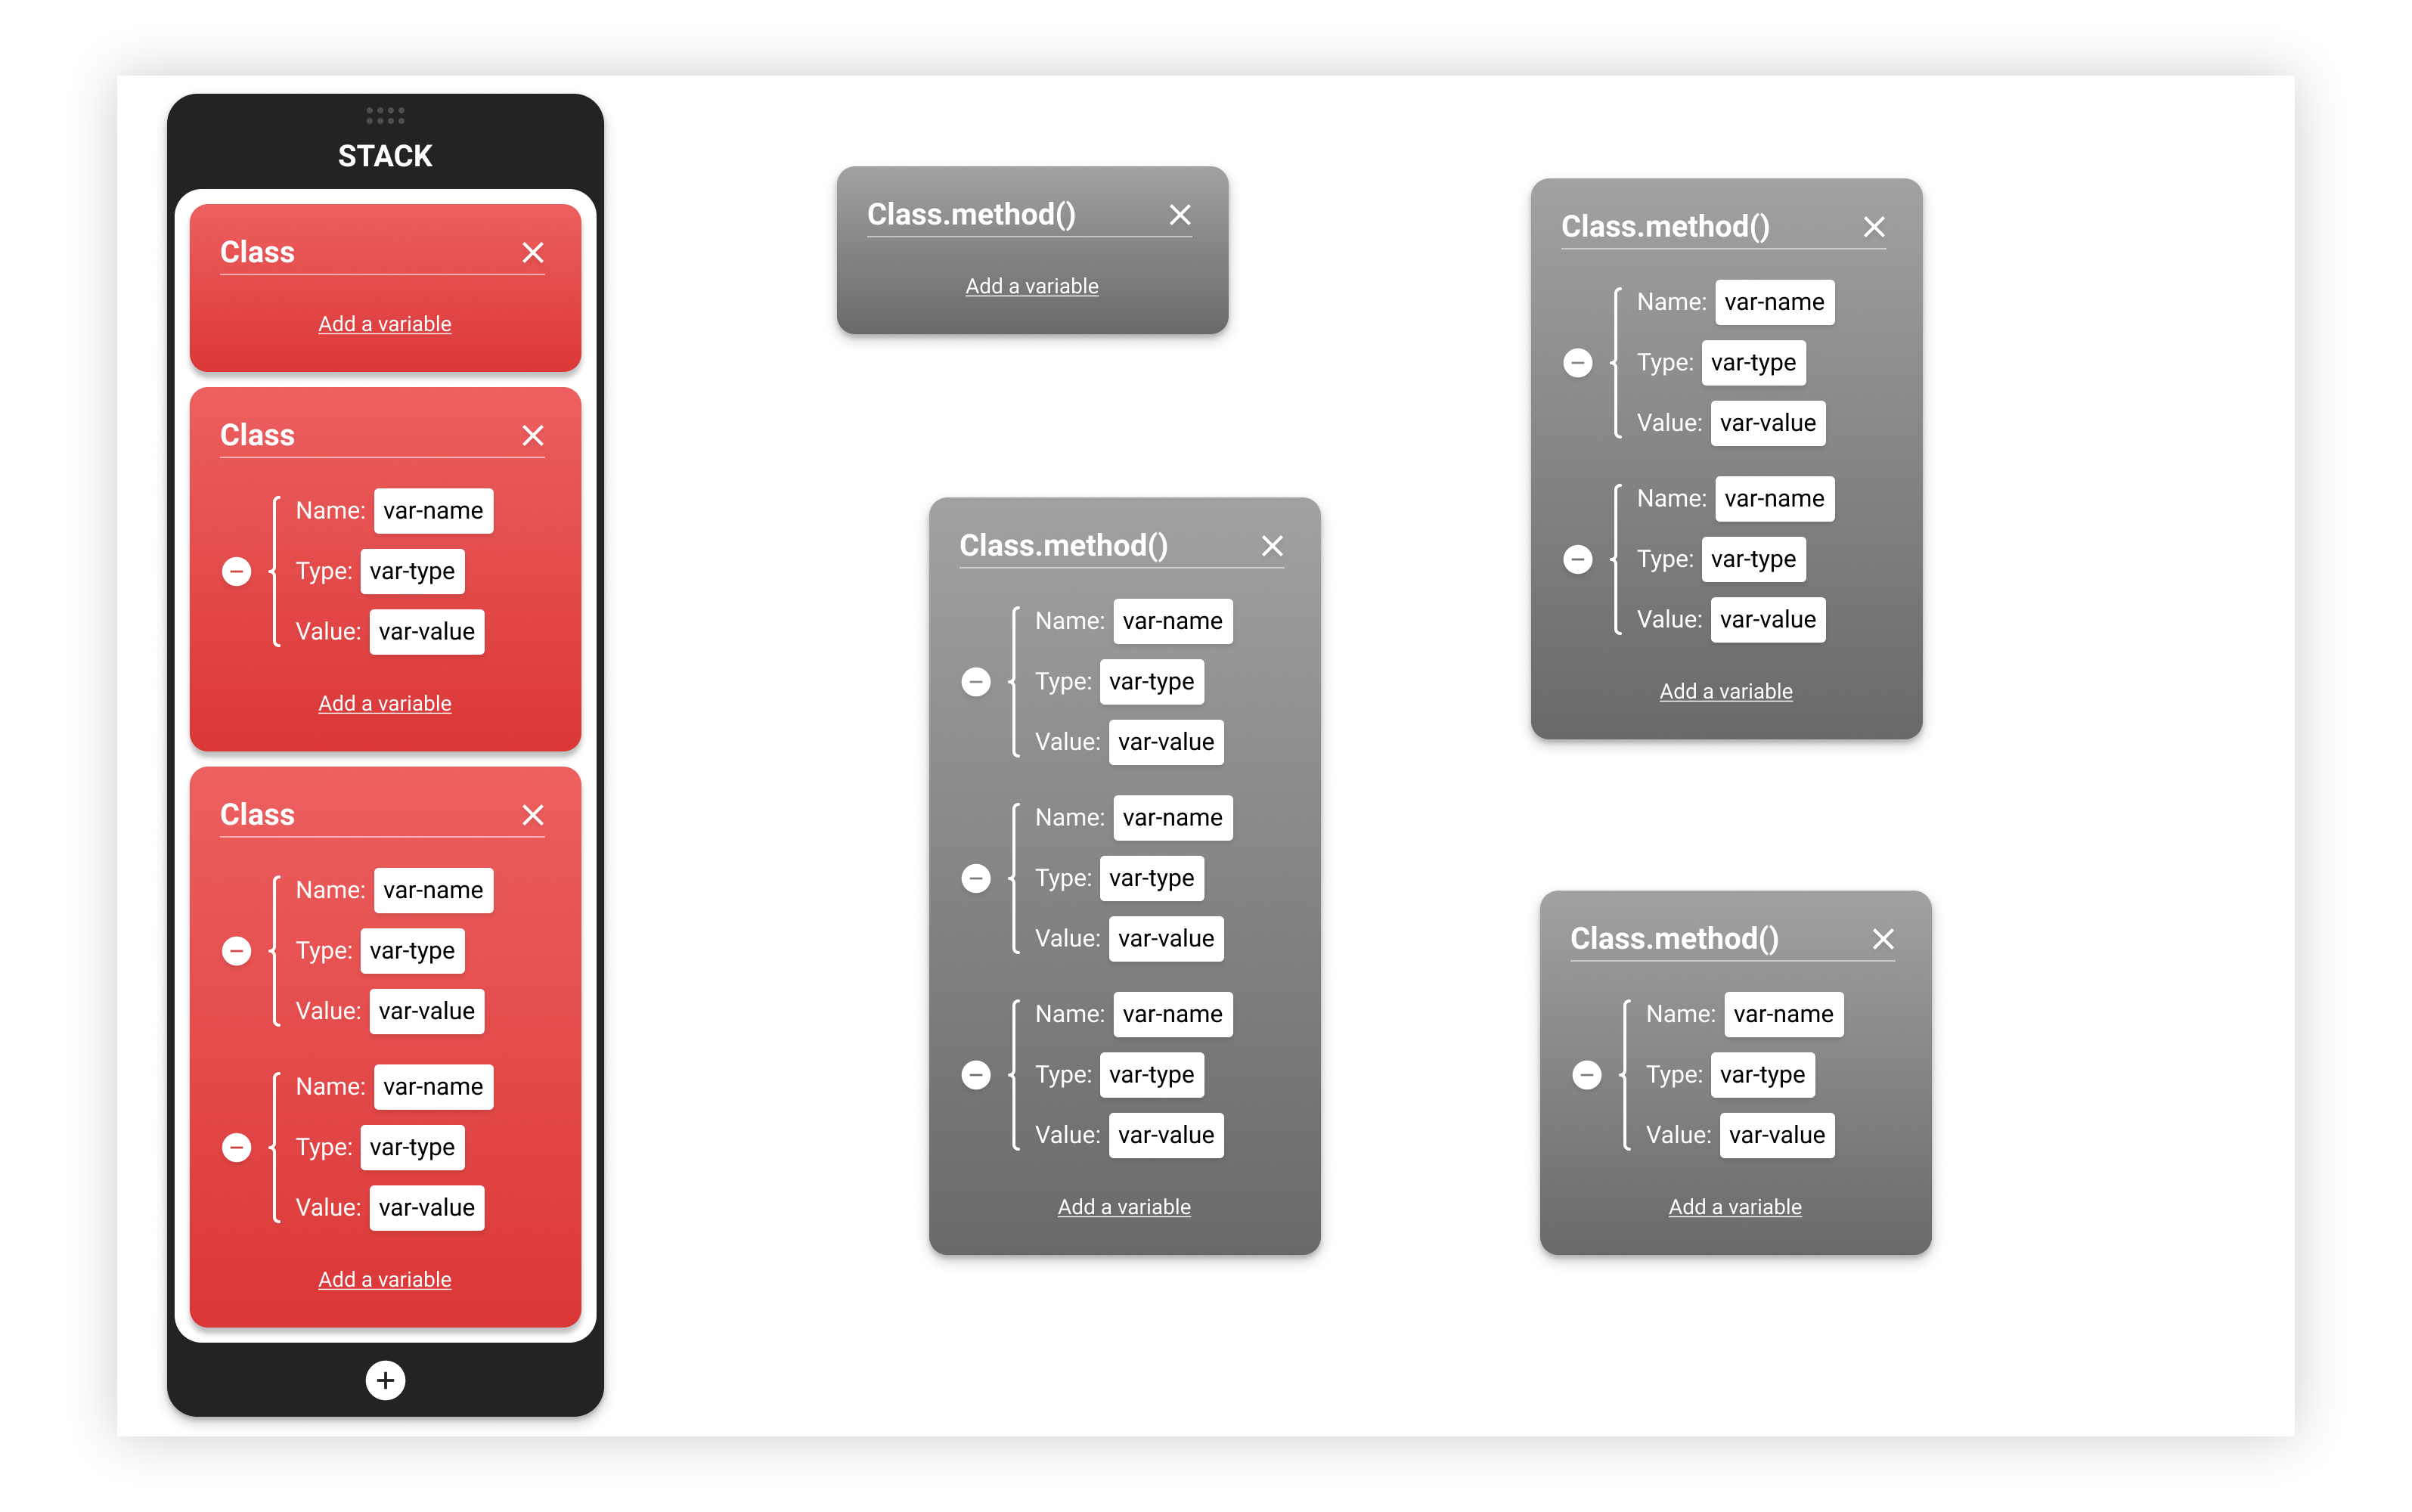
\includegraphics[width=\textwidth]{figures/floating_stack.png}
\caption {First version of the user interface, with a floating stack}
\label{floating stack}
\end{figure}

\pagebreak

\noindent \hyperref[separate regions]{\textbf{Figure 11}} shows an intermediate version of the design, which is substantially different from the previous one shown in \hyperref[floating stack]{\textbf{Figure 10}}. In fact, I tried to develop the idea of a docked stack. Actually, if compared to having it floating it might even have a few disadvantages, such as the impossibility of moving it around and occupying a fixed amount of space, which will not be available to the heap. On the other hand, it is stylistically a lot nicer on the eyes and it definitely delivers the best separation between the two regions. I also started playing with colors, in order to bring out a bit more playfulness from a rather schematic UI.\\
Besides stack and heap being separated by a divider, each has a header which labels the region where the user is working, and a plus button to add new stack frames and new heap objects.

\begin{figure}[h!]
\centering
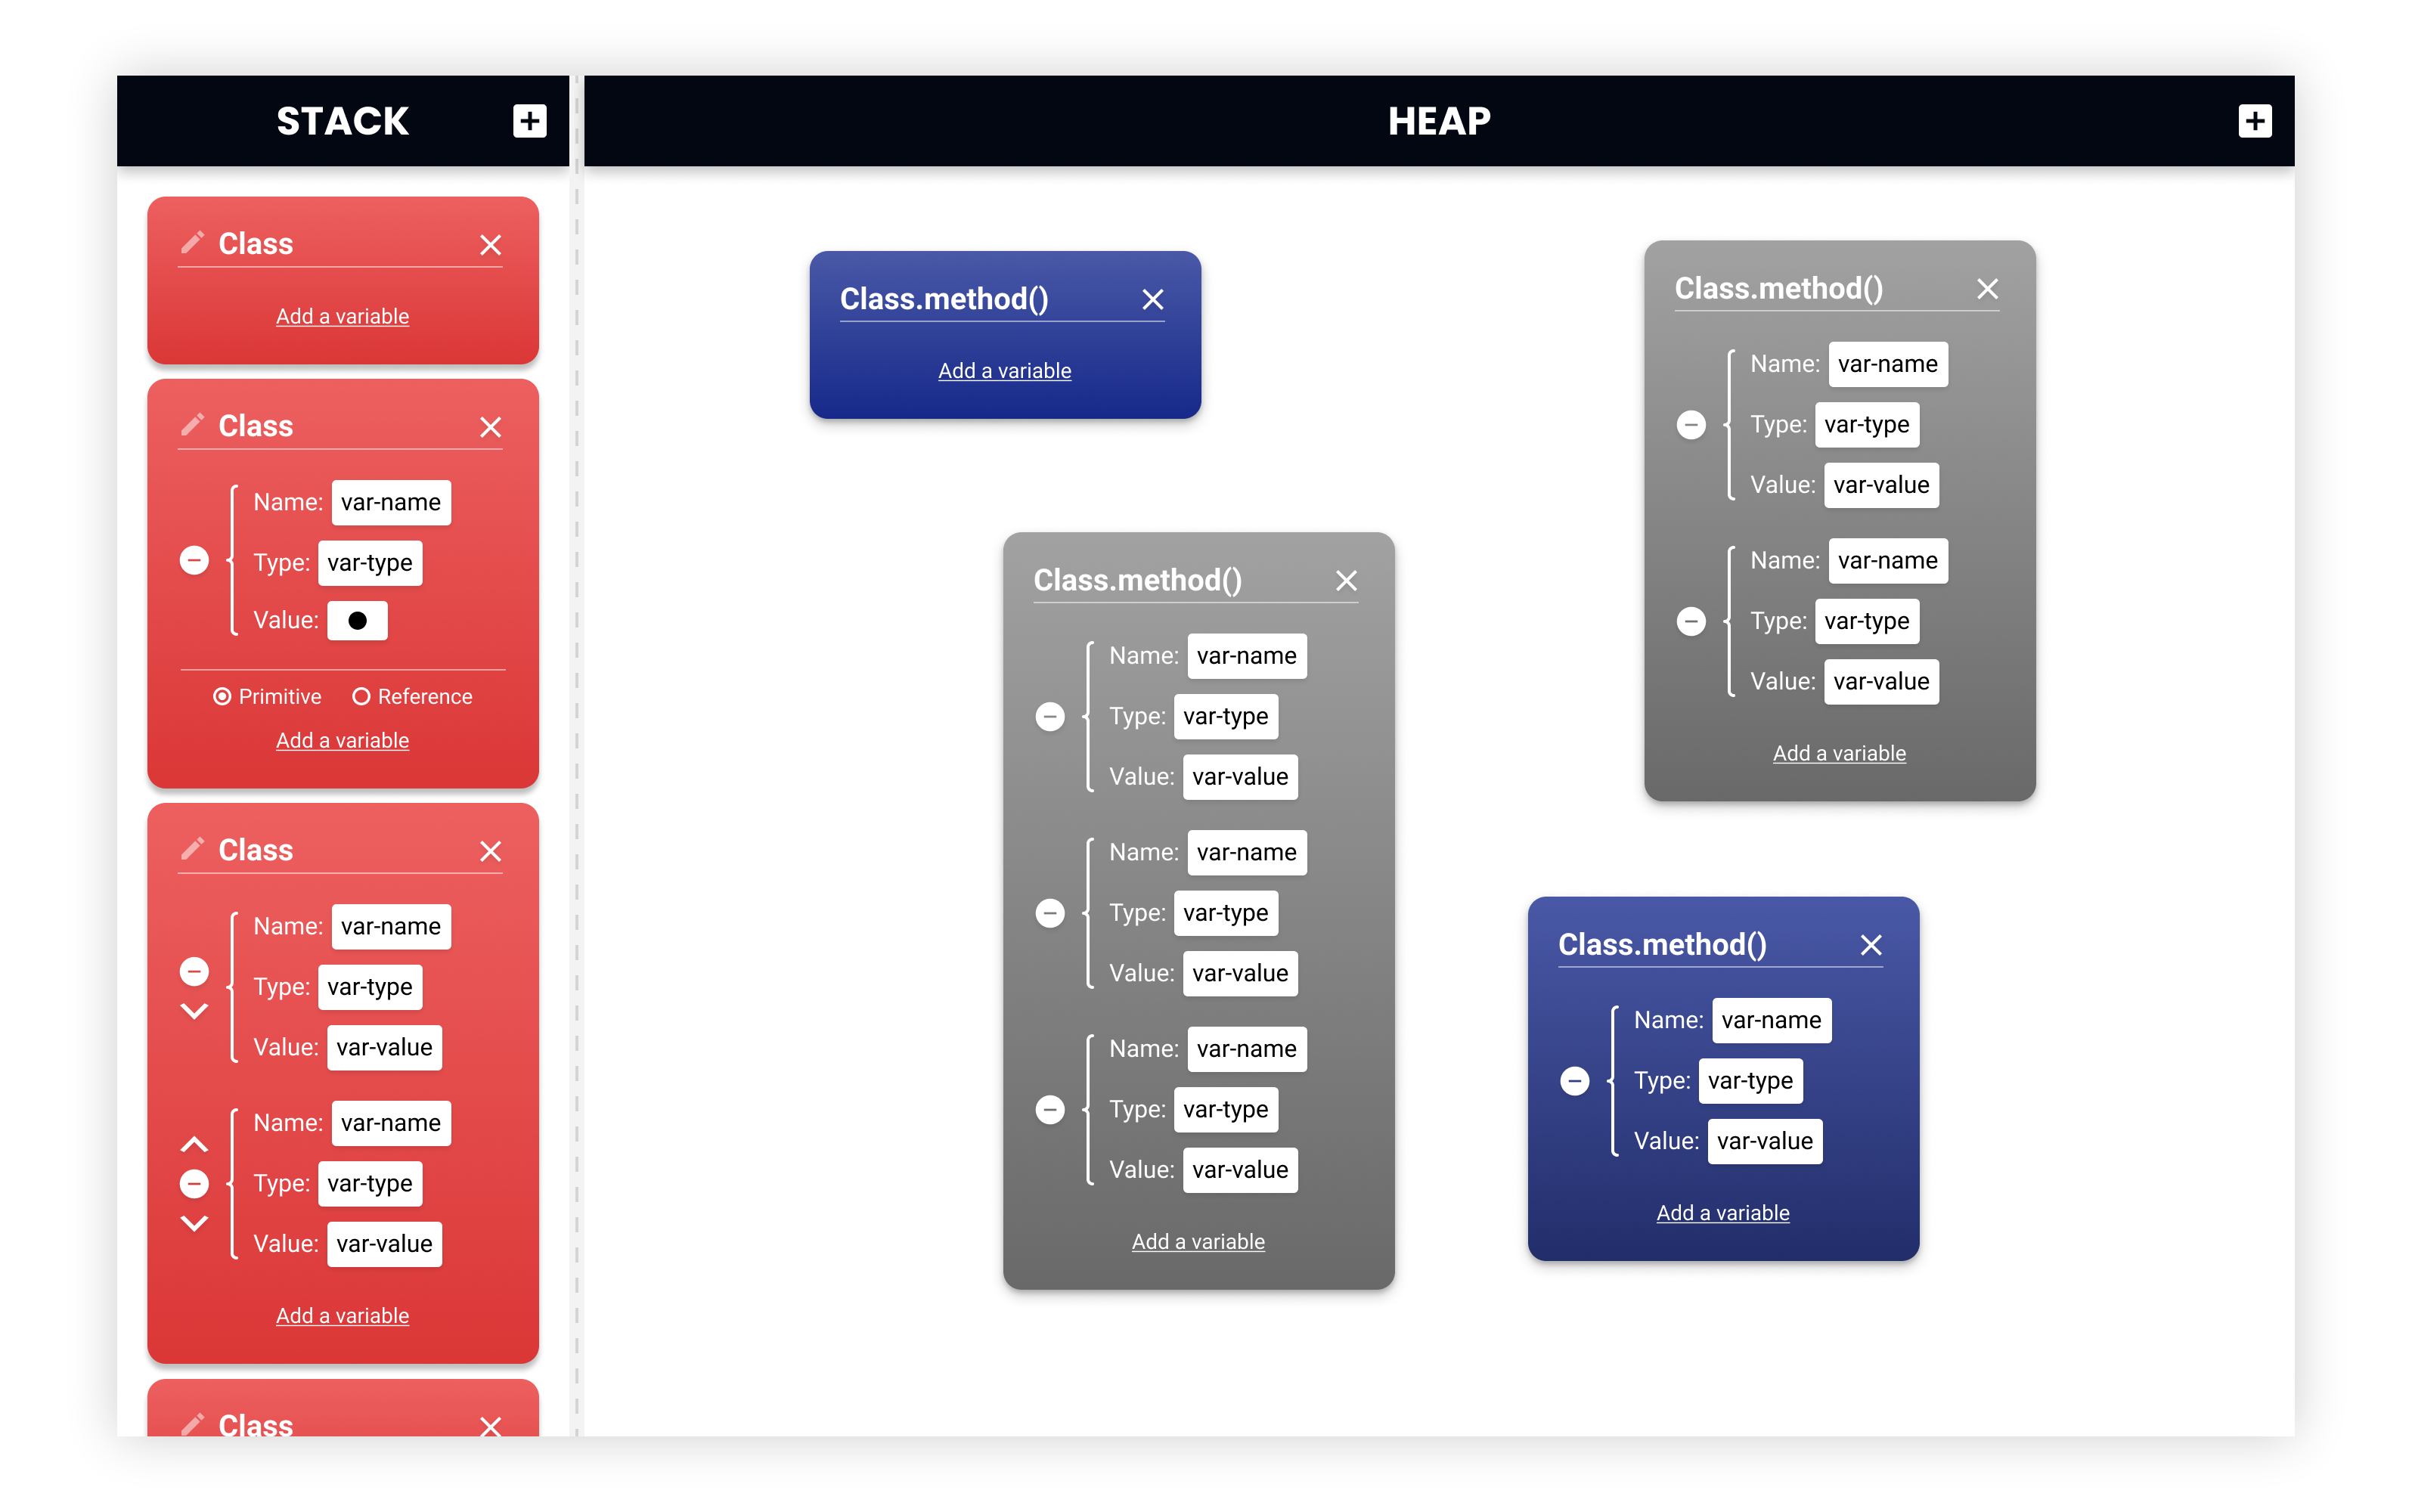
\includegraphics[width=\textwidth]{figures/separate_regions.png}
\caption {Intermediate version of the user interface with separate regions for stack and heap}
\label{separate regions}
\end{figure}

\noindent After several revisions, we eventually found a design solution which was good enough to continue with the rest of the development phase and you can see that in \hyperref[final ui]{\textbf{Figure 12}}. Compared to \hyperref[separate regions]{\textbf{Figure 11}} it presents some clear improvements, such as:

\begin{enumerate}
	\item Redesigned variables. Each one is now represented as a separate box inside the enclosing region block.
	\item Regions headers now display the number of blocks contained in it.
	\item Better color schemes.
	\item A toolbar is now docked on the right side of the window. It can be used to trigger some actions.
	\item Heap objects now have a handle at the top, so that users can drag them around.
\end{enumerate}

\noindent At this stage we have also started to notice how blocks were really big as opposed to the ones present in the clicker tool. However, we decided to keep this design because ultimately the pros outnumbered the cons and this issue could have been addressed during development.

\vspace{\fill}
\pagebreak

\begin{figure}[h!]
\centering
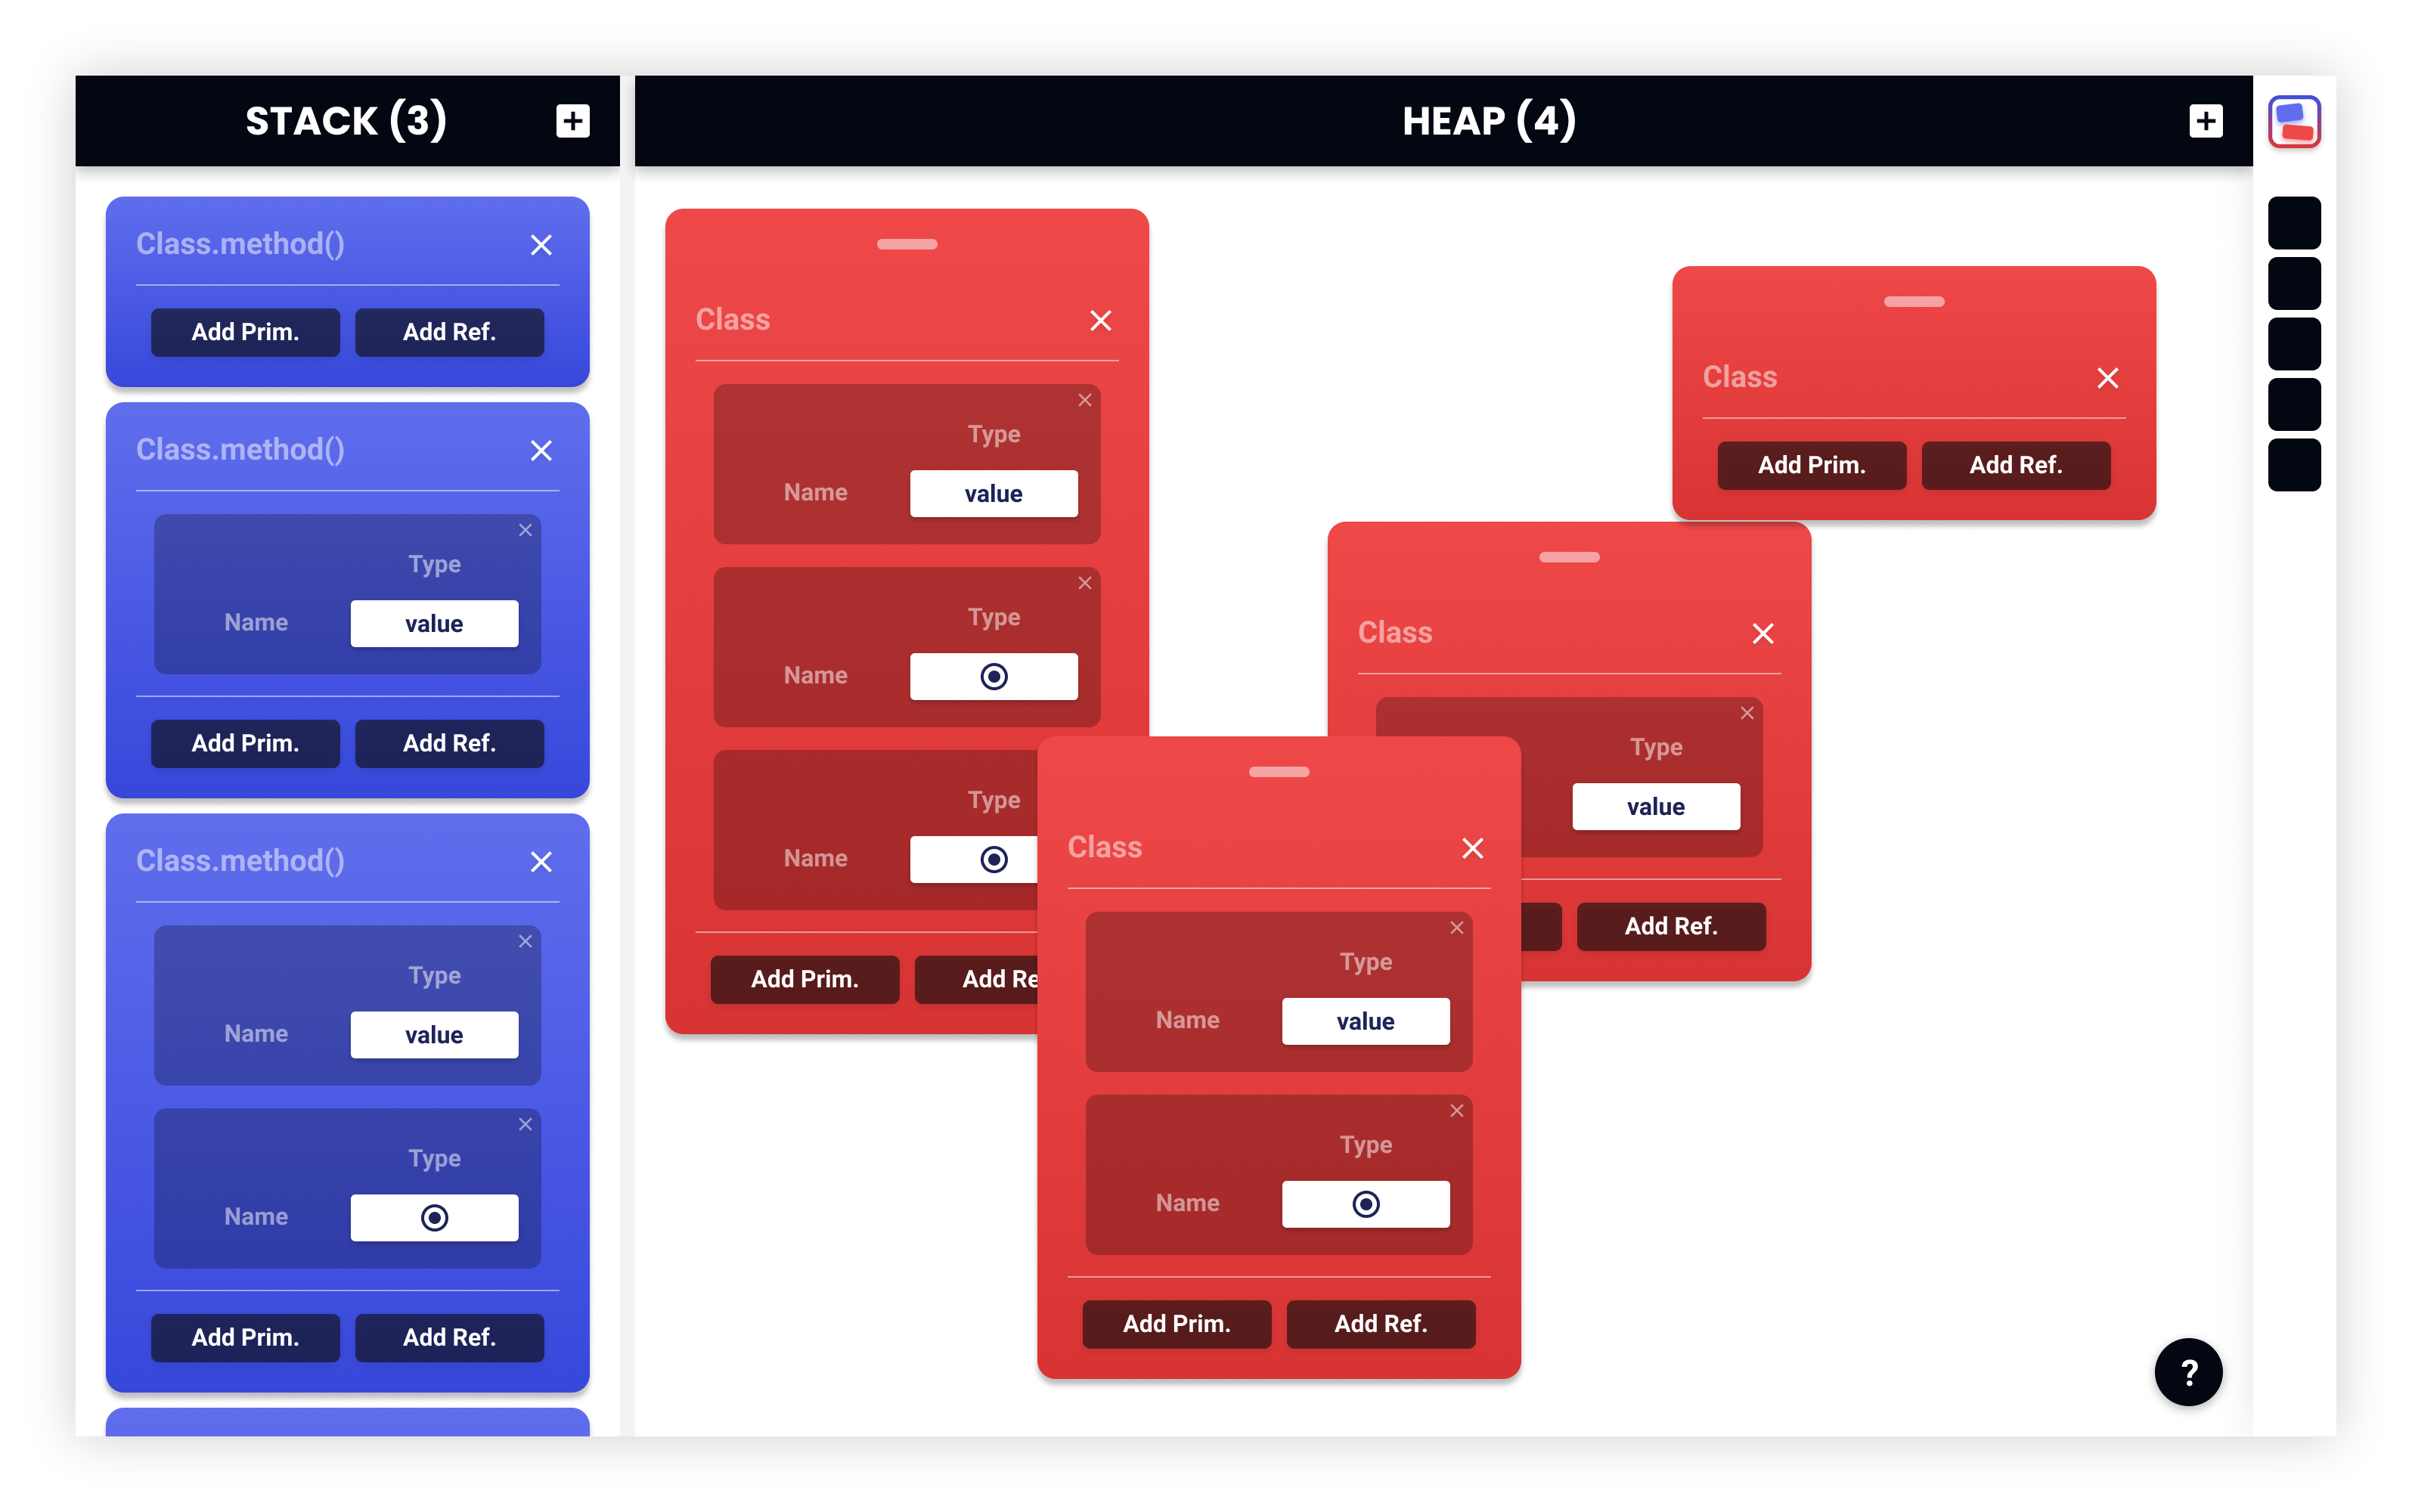
\includegraphics[width=\textwidth]{figures/final_mockup.png}
\caption {Final mockup of the user interface}
\label{final ui}
\end{figure}

\begin{figure}[h!]
\centering
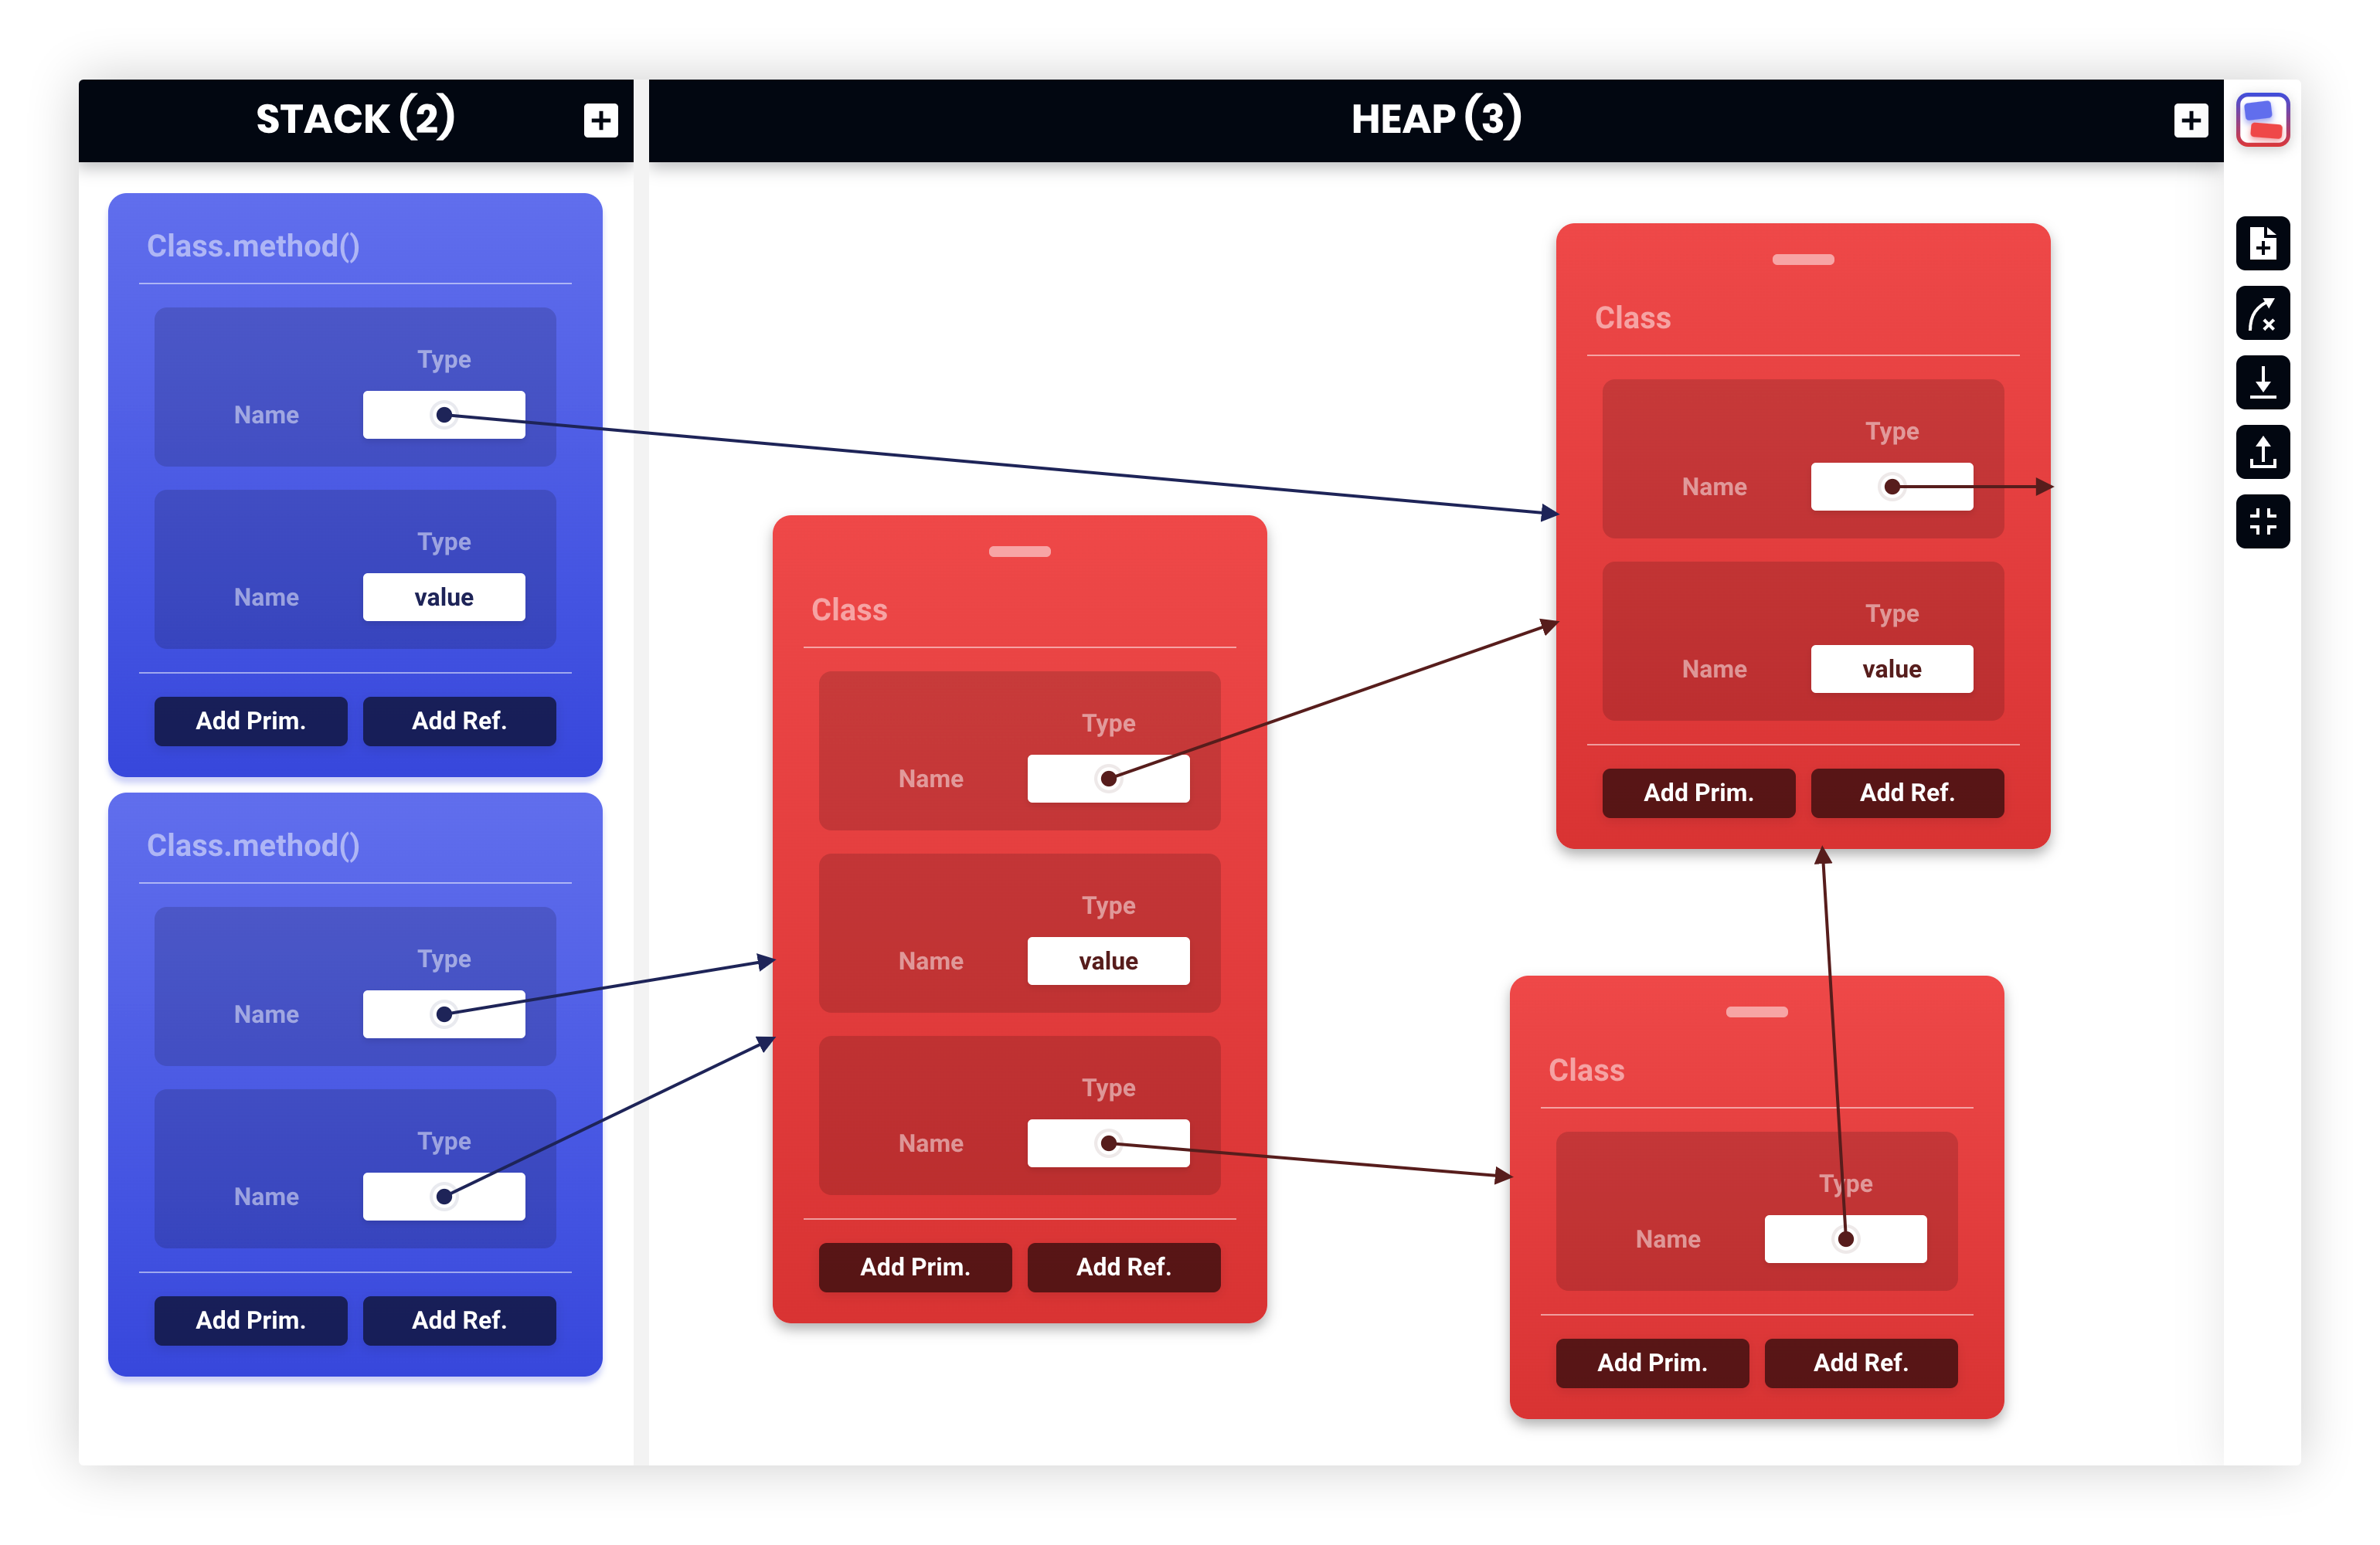
\includegraphics[width=\textwidth]{figures/final-interface.png}
\caption {Final interface of the web application at the end of the project}
\end{figure}
\subsection{Components tree}

Although stack and heap are separate regions that expect different user interactions, they share important similarities. In fact, they both:

\begin{itemize}
	\item Have a header, indicating the name of the area and the number of blocks that currently populate it.
	\item Have blocks, which look and function in the exact way, except their color schemes.
\end{itemize}

\noindent Because of these similarities, I have encountered some problems trying to extract the same features in common components in order to avoid as much code repetition as possible (see \hyperref[implementation]{\textbf{Section 5.3}}). \hyperref[tree]{\textbf{Figure 14}} shows the components tree on which I eventually settled.

\bigskip

\begin{figure}[h!]
\centering
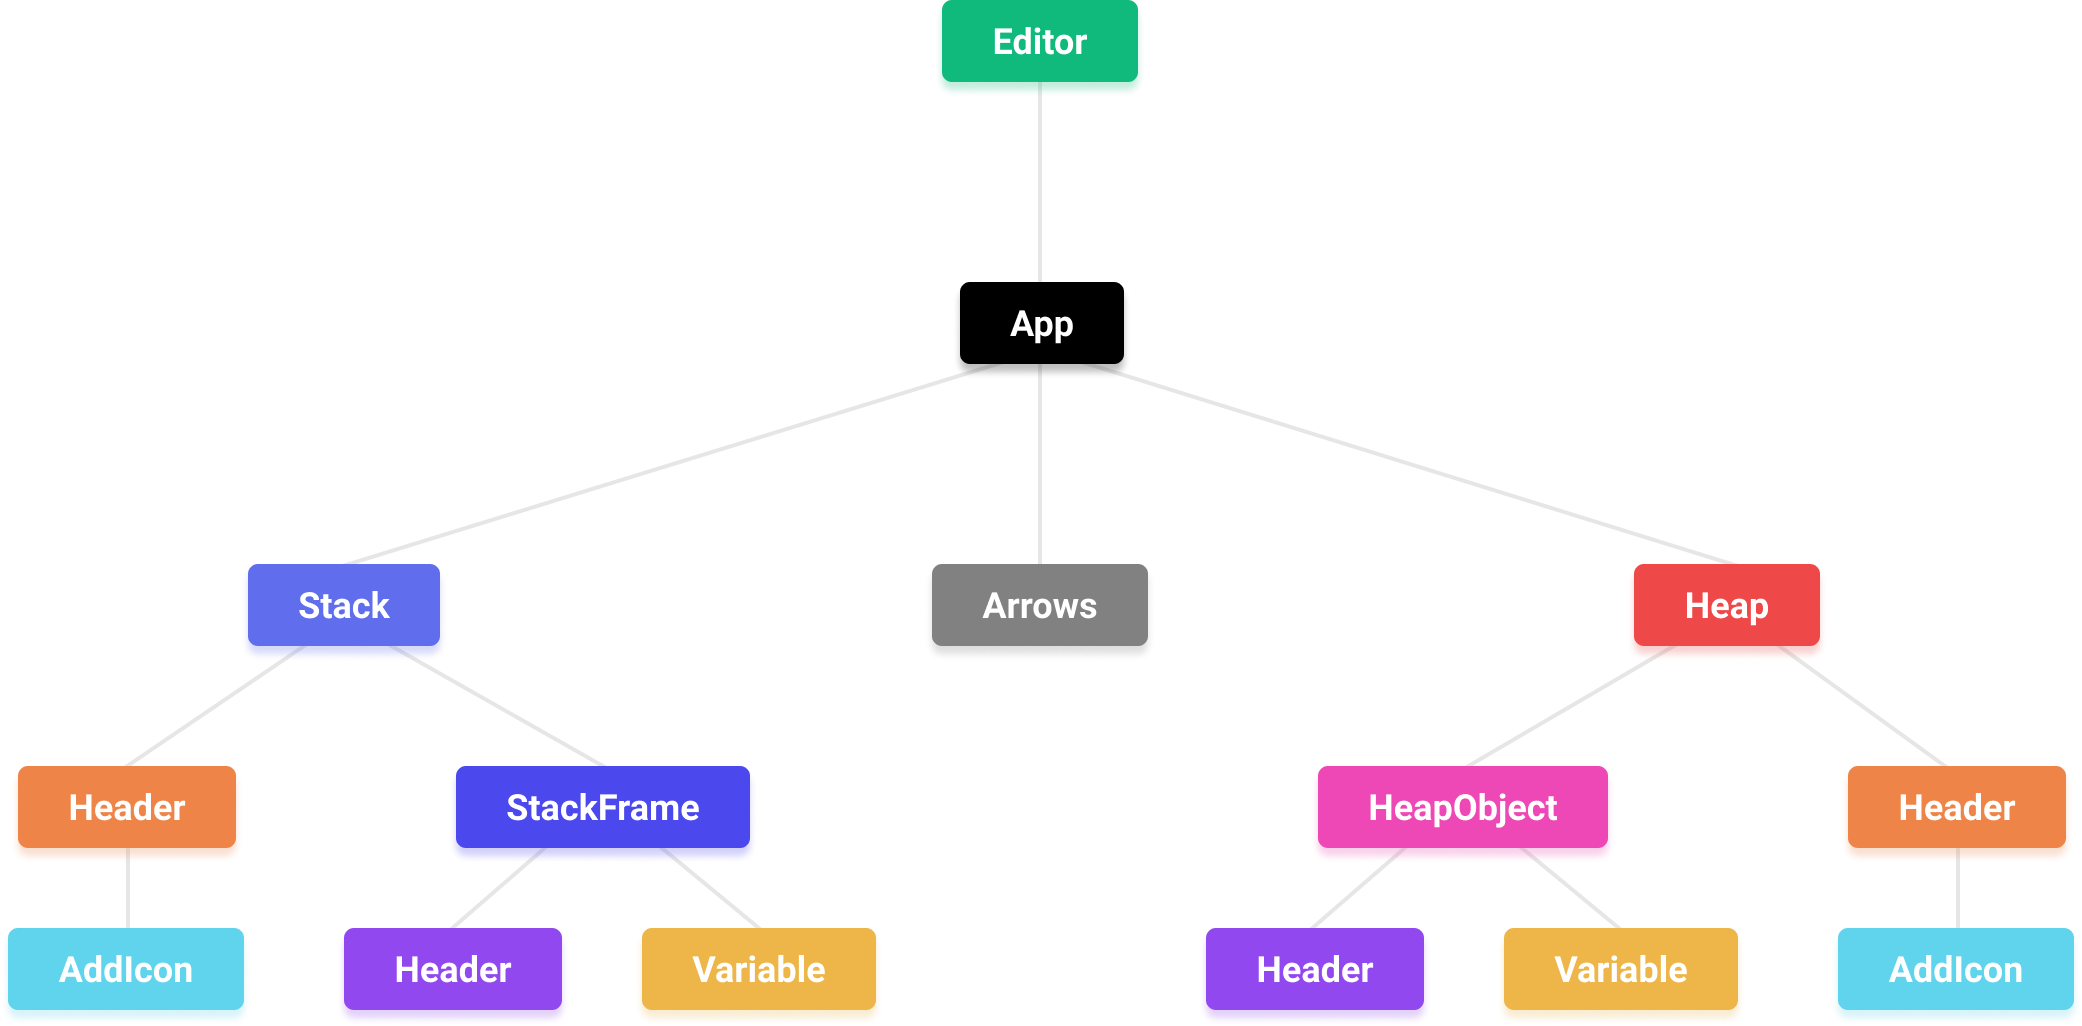
\includegraphics[width=\textwidth]{figures/tree.png}
\caption {Components tree visualization}
\label{tree}
\end{figure}

\bigskip

\noindent Starting from the top of the tree, \textbf{Editor} is the highest component. It is actually the component \textbf{App} wrapped in three context providers (more on this in \hyperref[storing states]{\textbf{Section 4.4}}), which allowed me to define global states across the interface. \textbf{App} is mainly used to define the layout of the web application, and some top-level computations, such as resizing the stack width, are done within this component.\\
Following the three branches, \textbf{Stack} and \textbf{Heap} are the components that represent the two areas of memory, and they keep and manage all the information related to their area within the application, while \textbf{Arrows} stores all the arrows present in the scene.\\
If we look at \textbf{\hyperref[tree]{Figure 14}}, we can really see how stack and heap are really similar. In fact, the only difference in their subtrees is the type of building block they can store. The stack stores \textbf{StackFrames}, while heap stores \textbf{HeapObjects}. They look very similar, but the data they generate is different (see \hyperref[json]{\textbf{Figure 15}}).\\

\begin{figure}[h!]
\centering
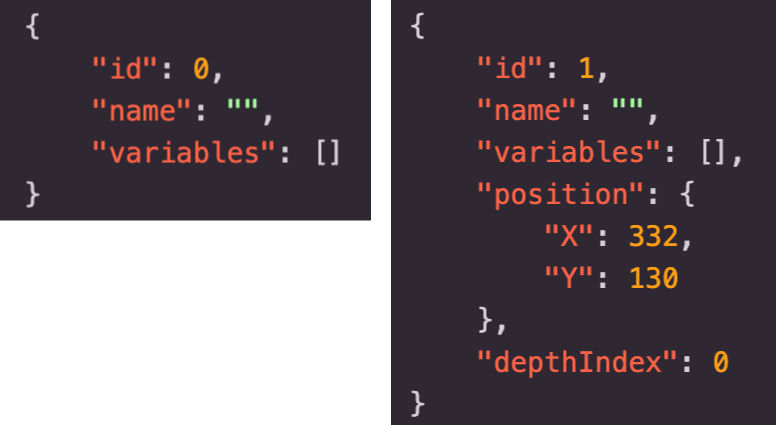
\includegraphics[scale=.3]{figures/blocks_data.png}
\caption {Snippet of the JSON file created by the web application, showing on left the data contained in a StackFrame, and on the right the data contained in a HeapObject}
\label{json}
\end{figure}

\noindent As we can see, heap objects have more data due to the fact that you can drag them around (hence the \emph{position}) and while doing so the one you are currently moving, goes on top of the other ones (hence the \emph{depthIndex}).\\
Going back to the components tree, every block has a \textbf{Header}, where users can write either the name of the class method name or the class name, and one or more \textbf{Variables}.\\
Both the stack and the heap have a \textbf{Header}, which shows the region name and the number of frames/objects created. Headers at the region level contain a component called \textbf{AddIcon}, which handles the creation of new blocks.

\vspace{\fill}
\pagebreak

\subsection{UI functionalities}

In this subsection I am going to walk you through every functionality that this stack and heap diagram editor offers to the user.\\

\ul{Stack}

\begin{itemize}
	\item Clicking on the plus button in the header, a new stack frame is created.
	\item Stack frames are always added at the top of the stack.
	\item When the stack contains more frames than the window can fit, the stack becomes scrollable. 
	\item The header renders the number of frames currently populating the stack.
\end{itemize}\

\ul{Heap}

\begin{itemize}
	\item Similarly to what happens in the stack, by clicking on the plus button, users can create new objects on the heap. However, the buttons works a bit differently: when it is yellow, the state is ``on'', the mouse cursor changes and the user can create a new object by clicking on the heap; when it is white, the state is ``off'' and the objects creation is disabled.
	\item Objects on the heap can be dragged around by clicking on their handle at the top.
	\item In the header it is rendered the number of objects currently populating the heap.
\end{itemize}\

\ul{Regions separator}

\begin{itemize}
	\item Users can drag horizontally the vertical separator between the stack and the heap to resize their width.
	\item Users can reset the stack width by double clicking on the vertical separator.
\end{itemize}\

\ul{Stack frames and heap objects}

\begin{itemize}
	\item Users can type the name of the class method that generated a given stack frame.
	\item Users can type the name of the class that generated a given object on the heap.
	\item Users can create primitive and instance (``reference'') variables.
	\item Users can fill the information of a variable, like the name, the type and the value.
	\item If a variable is of nature primitive, its value can be written using the keyboard.
	\item If a variable is of nature reference, an arrow is created by clicking on the circle icon within the value input field, holding the left mouse button and releasing it on a target object on the heap.
\end{itemize}\

\vspace{\fill}
\pagebreak

\ul{Toolbar}

\begin{itemize}
	\item Users can start a new project (all stack frames, heap objects and arrows are deleted).
	\item Users can delete all the arrows that have been created.
	\item Users can download a JSON file, representing the current state of the diagram.
	\item Users can upload a JSON file that was downloaded from the application. This file is parsed and it triggers the application to re-render with the state of the diagram at the time of downloading that file.
%	\item Users can scale up the interface. At every click, the base font-size (16px) is increased by 2px.
%	\item Users can scale down the interface. At every click, the base font-size (16px) is decreased by 2px.
	\item Users can go to and exit from fullscreen mode.
\end{itemize}

\subsection{Storing global states} \label{storing states}

In React, data is usually shared via props from parent to children: they can receive functions as props and send some data back to the parent using callbacks, but they cannot pass props back to the parent component.\\ Passing props through many levels is called \emph{props drilling} \footnote{\url{https://newreactway.com/what-is-prop-drilling-in-react/}}, and it is generally seen as a situation to avoid if props needs to traverse more than three levels of components. In fact, it becomes difficult for the developer to clearly understand what is going on, ending up storing data in intermediate components that are never going to use it.\\

\noindent Depending on the task, there are generally two approaches to solve (or at least improve) the situation:

\begin{enumerate}
	\item Composition
	\item State management tools (e.g., \emph{Redux} \footnote{\url{https://react-redux.js.org/}} and \emph{Context} \footnote{\url{https://reactjs.org/docs/context.html}})
\end{enumerate}

\noindent Both approaches have pros and cons, but for global data transferring it makes more sense to use a state management tool, which is what I did. I used the native React Context API in conjunction with the relatively new \emph{React Hooks} \footnote{\url{https://reactjs.org/docs/hooks-intro.html}}. By doing so, I have been able to access data from any level of components tree. However, I must also confess that Context, while being great at what it unlocks, introduces a bit of chaos when overused, which is sadly my case. This is maybe the aspect of this web application I would like to revisit the most in a few years, when I will be more experienced.\\

\noindent In particular I created the following contexts:

\begin{itemize}
	\item \ul{\emph{arrowsContext}}: used to store data about arrows.
	\item \ul{\emph{heapAddModeContext}}: it allows communication between the plus icon in the heap header and the heap dragging area, effectively allowing the user to freely create objects on the mouse position.
	\item \ul{\emph{heapDepthIndexContext}}: it allows me to keep always the current dragged heap object above the others, by correctly setting their CSS \emph{z-index} properties.
	\item \ul{\emph{heapMousePositionContext}}: in order to drag heap objects around, many different components needed to access the mouse position, so this context takes care of that.
	\item \ul{\emph{resizableStackContext}}: because of the layout of the application, resizing the stack causes many coordinates to be recomputed, involving components from different  parts of the components tree. This context allows all these elements to access the data they need.
	\item \ul{\emph{stateContext}}: this context stores all the data about the diagram and keeps a big JavaScript object updated with every state change happening in the application.
\end{itemize}

\vspace{\fill}

\pagebreak

%%%%%%%%%%%%%%%%%%%%%%%%%
\section{Implementation} \label{implementation}
%%%%%%%%%%%%%%%%%%%%%%%%%

In this section I am going to talk about some important aspects of the development process that were particularly challenging, and how I managed to find solutions in order to continue with the implementation of the design. The code base is hosted on a GitHub repository \footnote{\url{https://github.com/DaveKeehl/shd-editor}} and it is deployed on the Netlify servers \footnote{\url{https://stackandheap.netlify.app/}}.\\
\noindent In the near future, this web application will be embeddable on other React applications and all it is needed in order to do that, is to place the \textbf{Editor} component anywhere in the JSX. React will take care of the rest.

\subsection{Dragging}

One of the core features of the Informa clicker was the ability of being able to drag elements around the screen. When I was in the process of deciding how to implement it, I considered leveraging the \emph{draggable} attribute of HTML because it allows exactly that and it makes dragging very smooth, since it is supported by the browser out of the box. Moreover, there are many event listeners that one can use to customize the experience using React, naming the \textbf{onDrag}, \textbf{onDragStart}, \textbf{onDragEnd}, \textbf{onDragEnter}, \textbf{onDragExit}, \textbf{onDragLeave} and \textbf{onDragOver} events.\\
From the outside it might seem like a perfectly viable solution, however this method has a major drawback: the dragged element looks like a semi-transparent ghost clone of the original and you cannot apply any styles to it, as CSS does not provide any rules to target it. Furthermore, this so called \emph{ghost clone} is not even part of the DOM \footnote{\url{https://developer.mozilla.org/en-US/docs/Web/API/Document_Object_Model/Introduction}}, so you cannot dynamically add CSS classes to customize its look, and it sets a very aggressive bounding box \footnote{\url{https://en.wikipedia.org/wiki/Minimum_bounding_box}} around the dragged object (you can see in \textbf{Figure 16} how the drop-shadow is sharply cut in the corners, instead of spreading naturally).
For these reasons, I decided to rebuild the whole dragging system by myself, which led me to a series of problems that I have documented in this section.
 
\begin{figure}[h!]
\centering
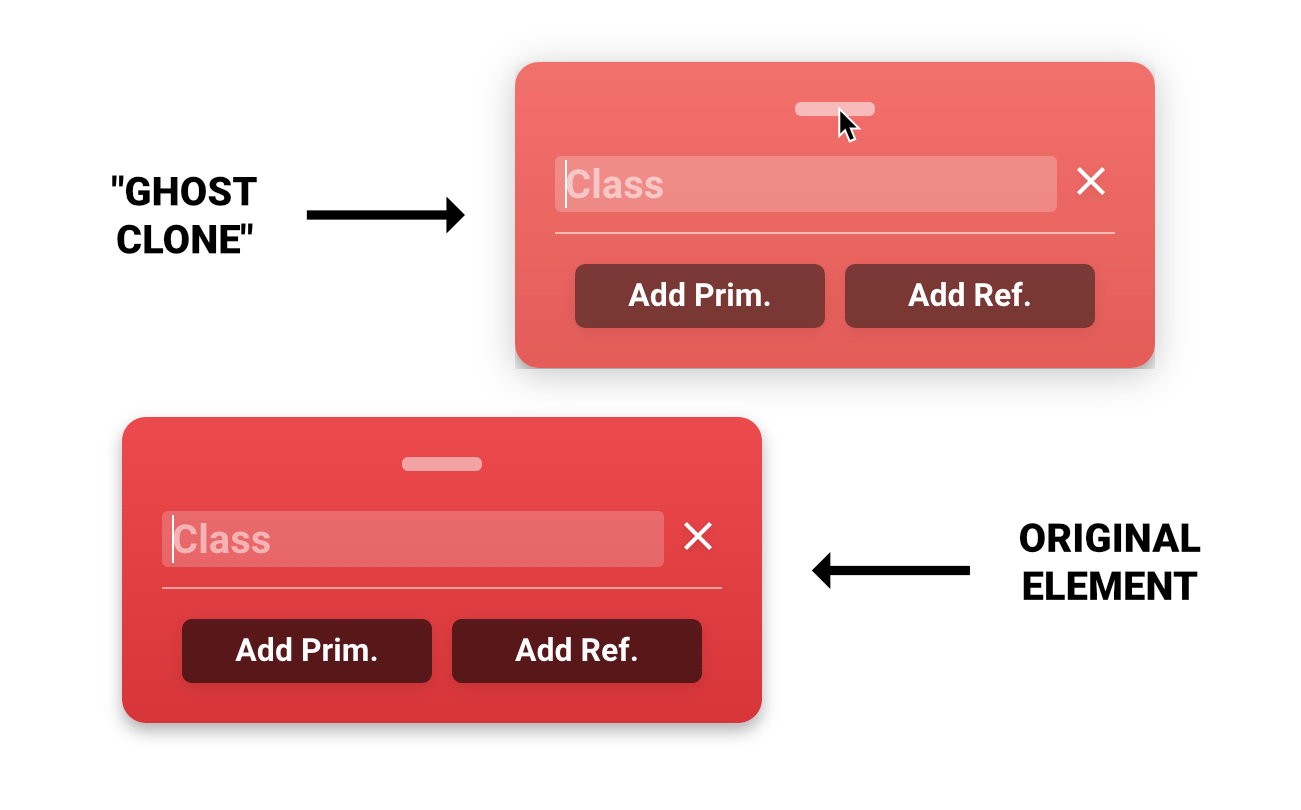
\includegraphics[scale=.5]{figures/ghost-clone.png}
\caption {Depiction of what happens when using the native \emph{draggable} attribute}
\end{figure}
 
\subsection{Multiple coordinates conversions}

At the beginning of the project, when I was building all the JSX and setting up all the CSS rules, I soon discovered that stack and heap needed different ``treatments''. The stack is built using flexbox with vertical direction, so the coordinates of each stack frame do not really matter, they just stack on top of each other. On the other hand, heap objects need precise coordinates in order to be placed on the screen. However, there is a twist: heap objects coordinates are \emph{relative}, meaning that position ${(0,0)}$ is the top left corner of the heap (header excluded), while mouse coordinates are absolute (= relative to the entire viewport).\\
Objects on the heap use relative coordinates because the stack is resizable: if an object on the heap had position absolute, it would stay in the same place while resizing the stack, not producing the desired effect of seeing everything shift; it would also go \emph{behind} the stack, a very undesirable side effect.\\
Because of that, I often found myself converting coordinates from system to system.

\subsection{Middle ground between dryness and modularity}

In this web app, some components are incredibly similar in terms of look, but slightly differ in behavior. When using modular frameworks like React, such a situation is not as trivial as one might think. It is very easy to create one single big component that uses conditional rendering in order to avoid code repetition. In my case, that is exactly what happened when I was building the interface and I had just started to work on the drag feature of the objects on the heap.\\ I started having problems when I realized that stack frames and heap objects needed different data representations (i.e. spatial coordinates and z-index values because the current dragged object has to be on top of the other ones). At that point, I had to decouple stack/heap and stack frames/heap objects and find a good compromise between having components with identical elements inside and keep a relatively high level of modularity.

\subsection{Arrows}

Arrows were the toughest feature to implement. Partially because they are implemented using SVG \footnote{\url{https://it.wikipedia.org/wiki/Scalable_Vector_Graphics}} (\emph{Scalable Vector Graphics}) and the syntax and some of its aspect are not very easy (like the \emph{path} attribute), but also because of their highly dynamic nature in the context of this web application. In fact, in order to render them, I needed to have at least a rudimentary system that would register all the information representing an arrow (start/end position, start region, variable and parent from where the connection was created, target object on the heap).\\For that reason, during the first week of work on them, the only way I could have any sort of validation was by constantly printing values on the console in the browser, and by taking and analyzing screenshots. After a while I became very fast and it did not take me long to check on a photo editor if something was correct or not. However, when a bug appeared, the debugging process was always very slow and tedious, because it was difficult to pinpoint the source of the problem.\\

\noindent Arrows were also a challenge when I had to decide where to place them exactly in the DOM. Since they need to be drawn and always be visible while doing so, it meant that in terms of stacking order along the z-axis, they needed to be over all the other UI elements in the diagram. If I set the \emph{z-index} accordingly in my stylesheet that would visually work, but it would make everything below this new top layer not interactive. The key in this case was to find the right \emph{pointer-events} \footnote{url{https://developer.mozilla.org/en-US/docs/Web/CSS/pointer-events}} attribute value (more specifically \texttt{pointer-events:visible}), in order to let the arrows take up the entire screen, but at the same time allow the user to still interact with the underlying elements where there are no arrows drawn.\\

\noindent Another implementation issue I had when working with arrows, was about the way I was updating already drawn arrows. In particular, the web application keeps track of two things:

\begin{enumerate}
	\item The new arrow that is being drawn on the screen.
	\item All the arrows that have already been drawn and that need to ``listen'' for certain events and be updated accordingly (for example, an object that they are connected to, changes its position or gets deleted). When a new arrow is created (the mouse click is released on a valid target block), it gets added to the array of existing arrows if there is not already an arrow with the exact same data. 
\end{enumerate}

\noindent And when it came down to keeping the arrows updated, I could follow two paths:

\begin{enumerate}
	\item Listen for every event that led to the arrow coordinates being recomputed, and do different and specific calculations based on the event that just happened.
	\item Use the state diagram as the single source of truth from which the array of arrows is built upon. This way leads to rebuild the whole array more or less every time the state of the diagram changes.
\end{enumerate}

\noindent Technically, the first approach is more performant, because it only updates the arrows that do really change. However, in such an application where students are required to create little diagrams, it is really unlikely to have so many elements that the performance starts to suffer so much that it becomes unusable. Furthermore, using a single source of truth is far easier to manage than watching for multiple events. Hence, I opted for the second way as a solution for this issue, with some parts using the first approach as well.


\vspace{\fill}

\pagebreak

%%%%%%%%%%%%%%%%%%%%%%%%%
\section{User evaluation} \label{Testing}
%%%%%%%%%%%%%%%%%%%%%%%%%

We are almost at the end of this report, and after talking about the design and the most important aspects of the implementation phase, I want to discuss the user evaluation process, which gave me useful insights on how my application behaves in the real world with real users.

\subsection{Methodology}

The main goal of the user evaluation was to try to see if users actually had an easier time using my web application compared to using the Informa clicker. I selected the two following diagrams and gave them to fifteen computer science students (all of them had already used the Informa clicker before), asking them to reproduce both of them using the two tools, and writing down the time needed to complete each task. My hypothesis was that on a grand-scale, my application would require less time because of all the improvements that I made based on the UI/UX research.

\begin{figure}[h!]
\centering
\begin{subfigure}{.5\textwidth}
  \centering
  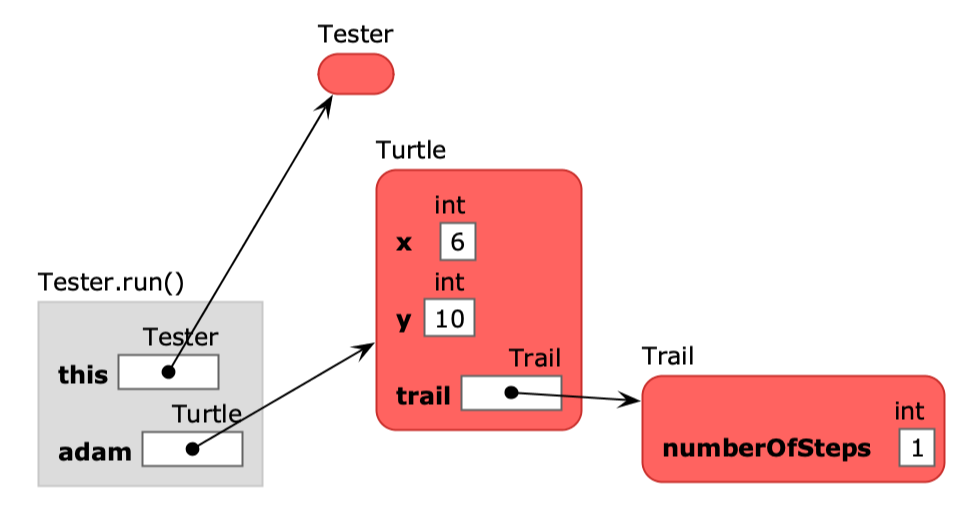
\includegraphics[width=\textwidth-10pt]{figures/informa_clicker_example2.png}
  \caption{Diagram 1}
\end{subfigure}%
\begin{subfigure}{.5\textwidth}
  \centering
  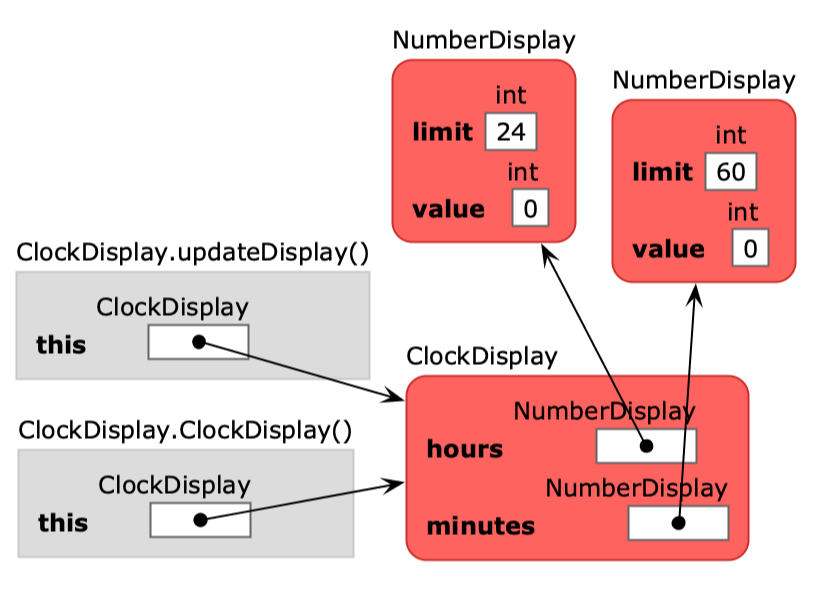
\includegraphics[width=\textwidth-10pt]{figures/informa_clicker_example4.png}
  \caption{Diagram 2}
\end{subfigure}
\label{fig:test}
\end{figure}


\noindent All participants had to do the same steps and in the same order. In this case, the measurements after drawing each diagram were to indicate the time required to draw each diagram. At the end of the experiment, the users were prompted to answer some final questions:

\begin{enumerate}
	\item Were you able to reproduce both diagrams? If not, why?
	\item Did you find the new application easier to use? If now, why?
	\item How would you rate the clarity of the layout in the new app (i.e. are all the features clearly laid out in an intuitive way or did you have to spend some time searching for them)?
	\item How would you rate the user experience in the new app (i.e. did something prevent you from successfully completing a certain task)?
	\item Did you experience any lag? If yes, how bad was it? Was it a problem for completing the task?
	\item Did you find any bugs? If yes, what bugs did you find? Could you list all the steps to reproduce them?
	\item Do you have any suggestions for improving the user interface and/or the user experience?
\end{enumerate}

\noindent With all the data, I created some graphs and did some statistics in order to properly assess the results.


\begin{figure}[h!]
\centering
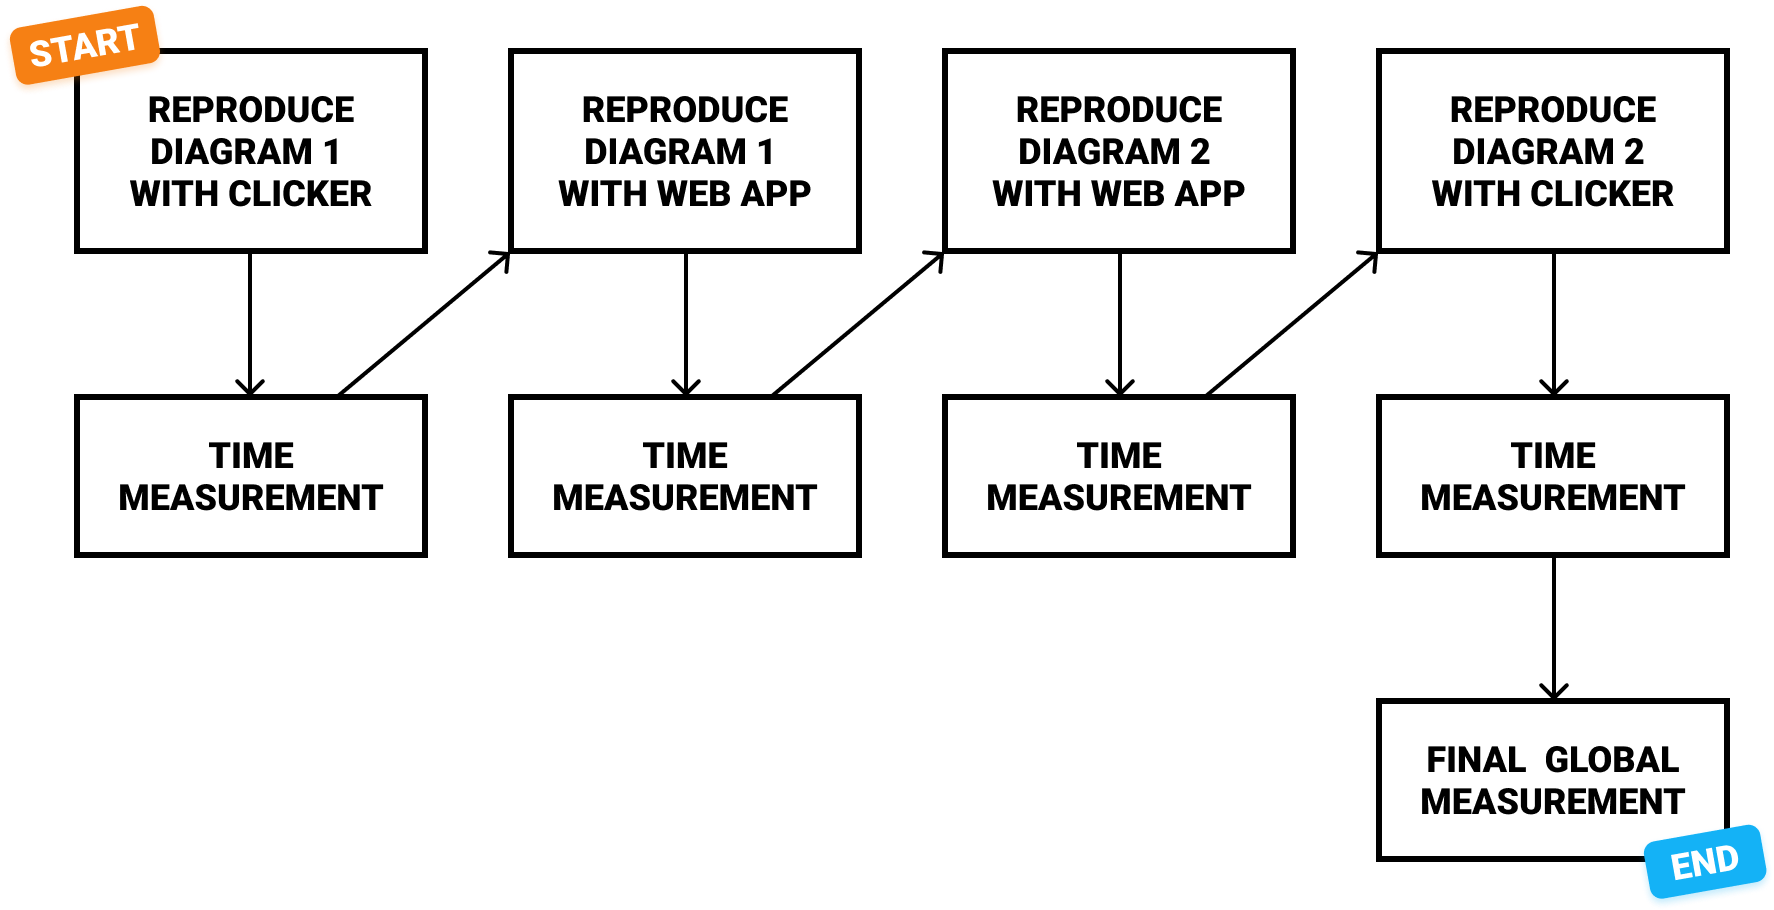
\includegraphics[width=\textwidth-50pt]{figures/experiment-design.png}
\caption {Design of the user evaluation experiment}
\end{figure}

\vspace{\fill}
\pagebreak

\subsection{Results}

All the participants were able to complete all tasks and (almost) everybody agreed on the fact that the new application is easier to use compared to the Informa clicker (see \textbf{Figure 19}), but if we look at \textbf{Figures 20} and \textbf{21} depicting the time duration it took them to reproduce the two diagrams, there are some interesting points to make.

\begin{figure}[h!]
\centering
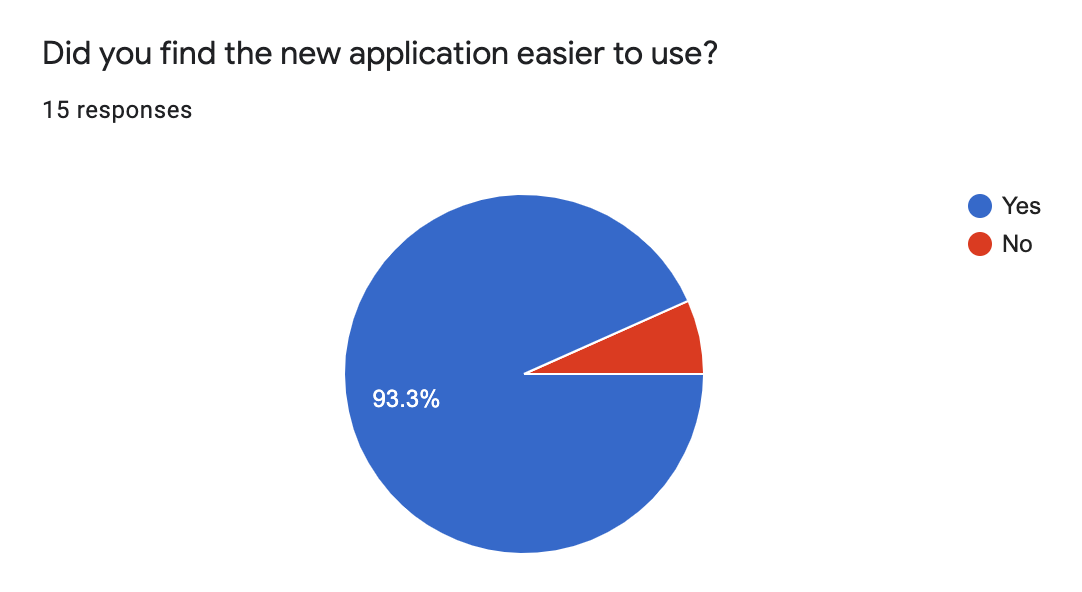
\includegraphics[scale=0.45]{figures/ease-of-use.png}
\caption {The majority of the participants found that the new tool is easier to use}
\end{figure}

\bigskip

\noindent As we can see in \textbf{Figure 20}, all participants were quicker to draw the diagram using the web application, but the same cannot be said for the second one. In fact, in \textbf{Figure 21} the situation is a lot more mixed and it is difficult to understand at first sight what exactly happened. However, after talking to all the participants and after reading all the answers to the question \emph{``Do you have any suggestions for improving the user interface and/or the user experience?''}, I realized that there were four problematic factors:

\begin{enumerate}
	\item Lack of advanced object manipulation, such as duplication and position shifting in the stack (moving stack frames up and down).
	\item Lack of navigability in the heap, combined to the elements being too big for the given space.
	\item Objects on the heap can only be dragged by clicking on the handle at the top of their shape. This creates problems when objects are stacked on top of each other and they cover the handle of the underlying elements, making it impossible to reposition them.
	\item The objects are too big and take up too much space
\end{enumerate}

\noindent All the answers from that final question were about one of those four points, so they are definitely to implement/fix in the future. I was aware of problems 2 and 3, but to be honest I had not even thought about the first one. Furthermore, the second diagram was busier than the first one and it required more elements in the scene, so it made sense that some issues would arise. I would have been surprised if the opposite happened.\\
However, despite the apparent mixed results of the second diagram, thanks to a straightforward statistical analysis, I was able to assess that the new web application scored higher nonetheless. In fact, 9 out of 15 people (60\%) were quicker with it, and both the average and median time duration needed to draw the diagrams using the web tool were lower than the Informa clicker counterparts. 

\begin{figure}[h!]
\centering
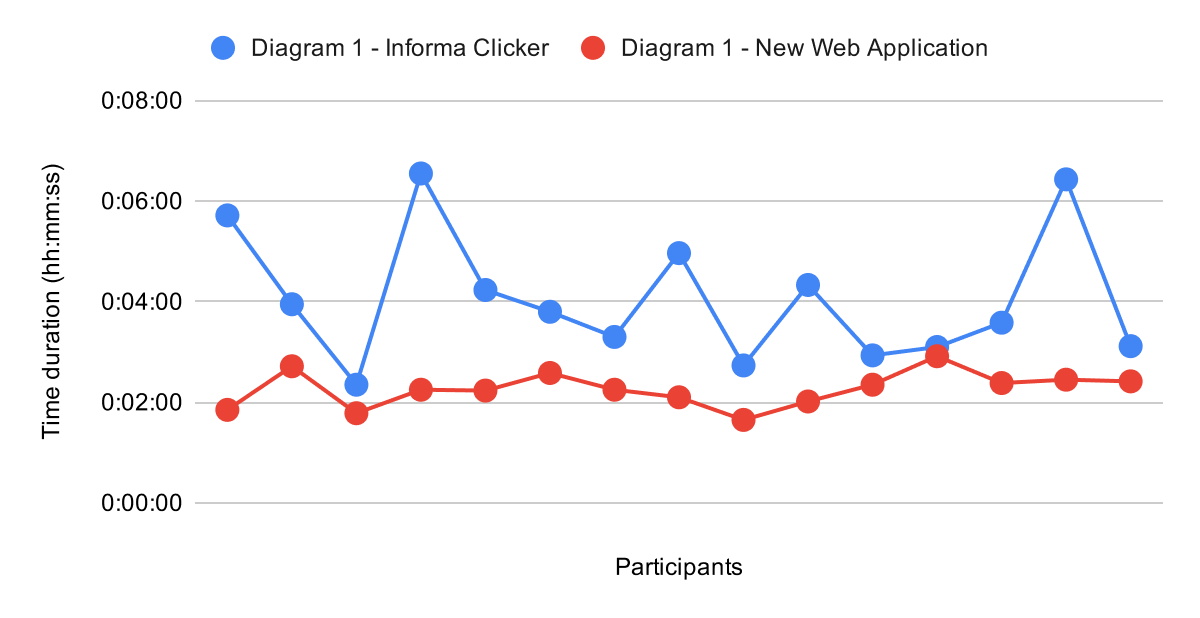
\includegraphics[scale=0.6]{figures/diagram1-time-comparison.png}
\caption {Diagram 1 - Time duration comparison between the Informa clicker and the new web application}
\end{figure}

\begin{table}[h!]
\centering
\begin{tabular}{|l|l|l|l|l|l|l|}
\hline
 & \textbf{Diagram 1 (Informa Clicker)} & \textbf{Diagram 1 (Web Application)} \\ \hline
\textbf{Average time duration} & 00:04:09 & 00:02:15 \\ \hline
\textbf{Median time duration} & 00:03:53 & 00:02:15 \\ \hline
\end{tabular}
\caption{Time duration comparison for the first diagram using the two tools}
\end{table}

\noindent As we can see in \textbf{Table 2}, the time duration difference needed to construct the second diagram using the two tools is not as big as for diagram 1, but it was still enough to assess my work positively. Moreover, it is also important to consider that while replicating the second diagram, many participants admitted that at that point they had grasped how the Informa clicker worked, and so they did not get lost like the first time. That is a clear indication that I have made a relatively good job at creating an intuitive interface.

\begin{figure}[h!]
\centering
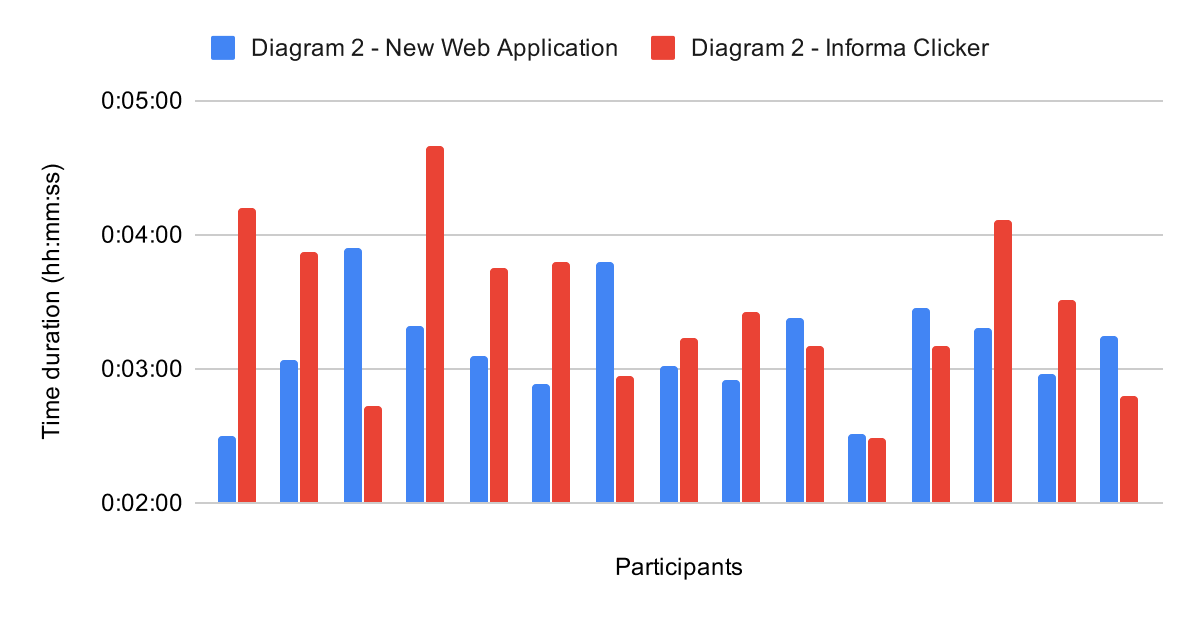
\includegraphics[scale=0.6]{figures/diagram2-time-comparison.png}
\caption {Diagram 2 - Time duration comparison between the Informa clicker and the new web application}
\end{figure}

\begin{table}[h!]
\centering
\begin{tabular}{|l|l|l|l|l|l|l|}
\hline
 & \textbf{Diagram 2 (Informa Clicker)} & \textbf{Diagram 2 (Web Application)} \\ \hline
\textbf{Average time duration} & 00:03:30 & 00:03:09 \\ \hline
\textbf{Median time duration} & 00:03:28 & 00:03:05 \\ \hline
\end{tabular}
\caption{Time duration comparison for the second diagram using the two tools}
\end{table}

\vspace{\fill}
\pagebreak

\noindent In addition to the time duration, I also I asked how much they would rate the clarity of the new layout and the user experience inherent from it. The participants gave positive feedback, leaving very high scores. \textbf{Table 3} shows the average and median scores, while \hyperref[clarity]{\textbf{Figures 22}} and \hyperref[ux-ratings]{\textbf{23}} show the exact ratings that were given.\\
It is also important to note that no participant had any problem in terms of lag.

\begin{figure}[h!]
\centering
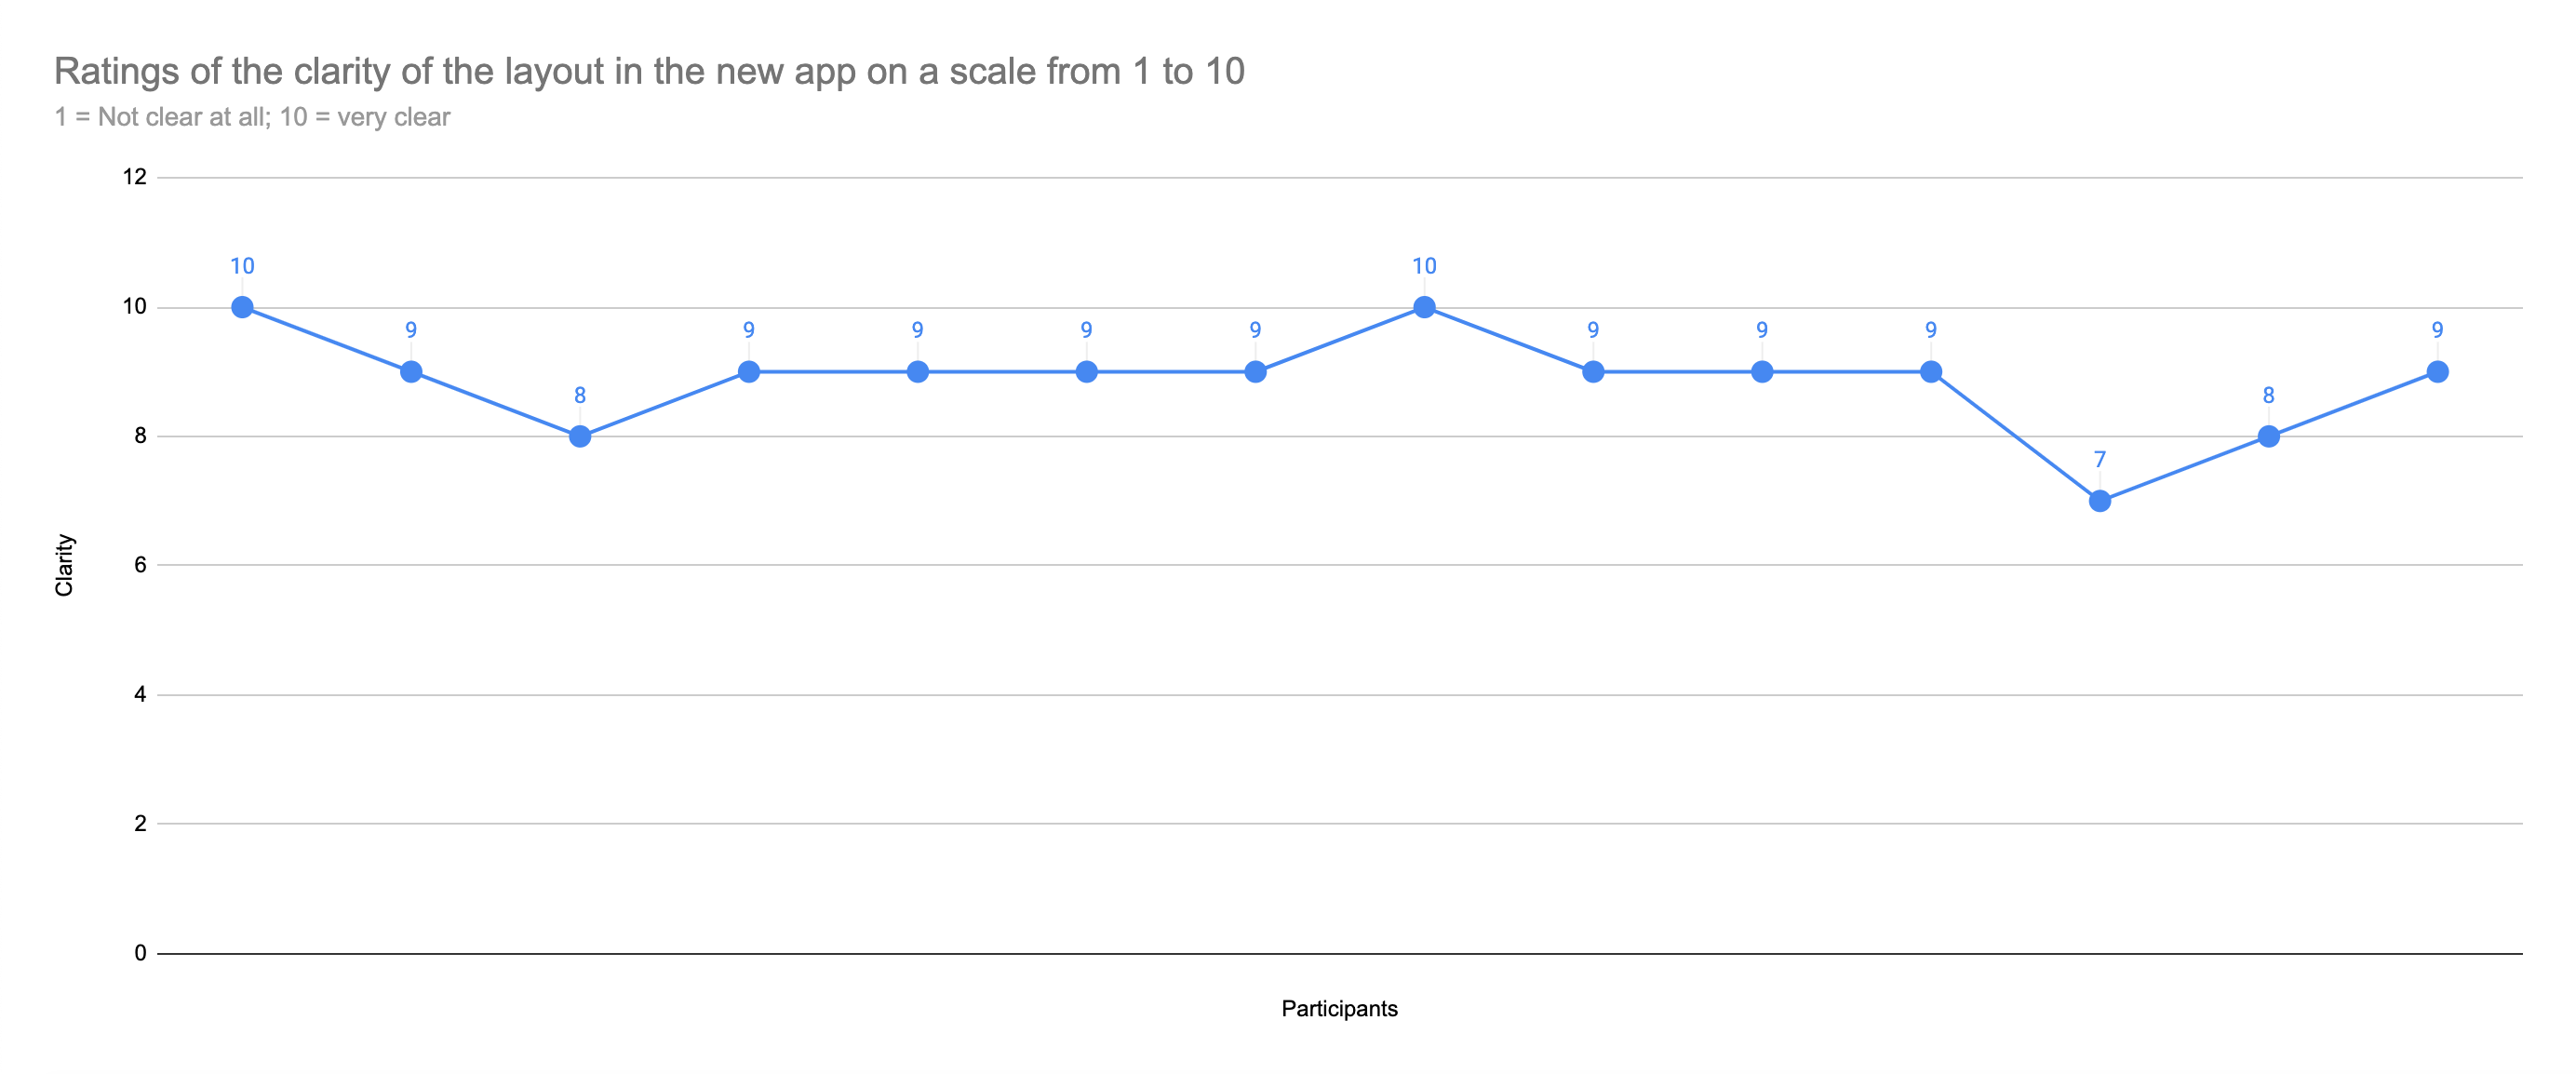
\includegraphics[scale=0.6]{figures/clarity-ratings.png}
\caption {Ratings of the clarity of the layout in the app on a scale from 1 to 10 (1 = not clear at all; 10 = very clear)}
\label{clarity}
\end{figure}

\begin{figure}[h!]
\centering
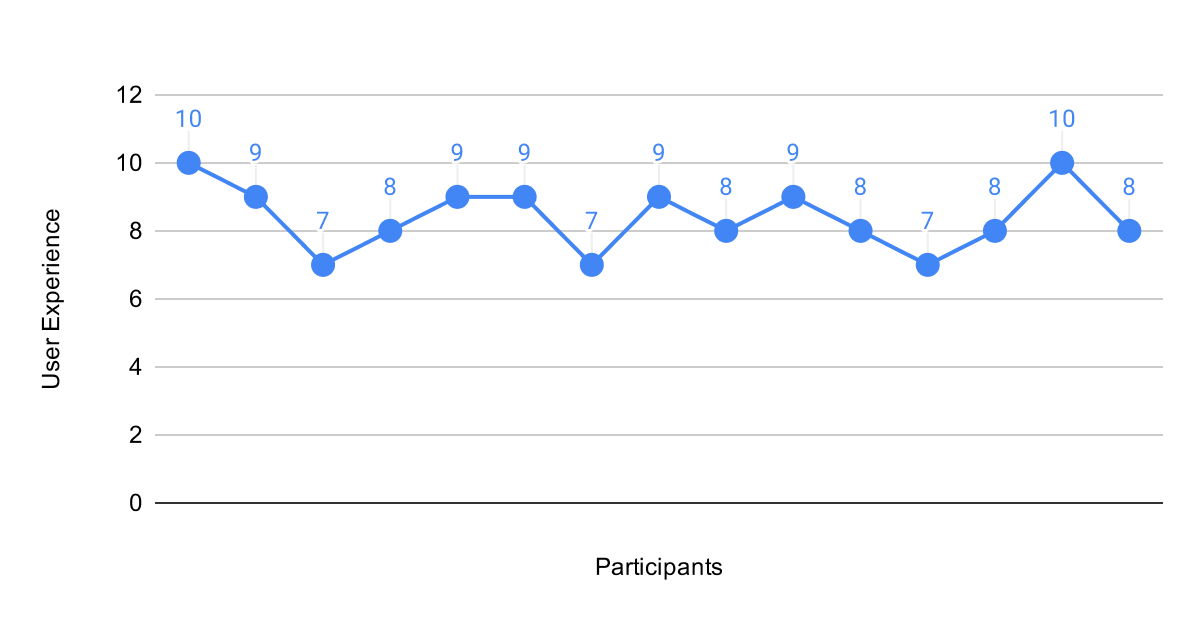
\includegraphics[scale=0.6]{figures/ux-ratings.png}
\caption {Ratings of the user experience in the new app on a scale from 1 to 10 (1 = terrible; 10 = amazing)}
\label{ux-ratings}
\end{figure}

\begin{table}[h!]
\centering
\begin{tabular}{|l|l|l|}
\hline
 & \textbf{Clarity ratings} & \textbf{UX ratings} \\ \hline
\textbf{Average} & 8.75 & 8.33 \\ \hline
\textbf{Median} & 9 & 8 \\ \hline
\end{tabular}
\caption{Average and median values of the ratings on a scale from 1 to 10 given by the participants to the clarity of the UI and to the general UX of the application}
\end{table}

\subsection{Comments}

Based on the results obtained by the user evaluation, I can say that users found the new web application easier to use, even if there are aspects that need to be perfected or further implemented in order to be fully considered ready for the public. Hence, my hypothesis can be considered accepted.

\vspace{\fill}
\pagebreak

%%%%%%%%%%%%%%%%%%%%%%%%%
\section{Conclusions} \label{Conclusions}
%%%%%%%%%%%%%%%%%%%%%%%%%

In this section I am going to assess my work and provide a list of features and improvements that one could work on in order to further extend the application.

\subsection{Personal assessment}

Now that the project is concluded, it is time for me to make some final assessments based on the end product that I have created. \\
In terms of features, I was able to complete all the minimum requirements, which means that my web application can replicate all the basic functions that were already possible in the Informa clicker. I have also implemented features that were not originally there, such as multi arrow selection/deletion, upload and download of JSON files and fullscreen mode.\\
In terms of performance the results are good, but there is some margin of improvement. Having to constantly capture the mouse position is expensive, but it is unfortunately required to do any coordinate computation. In fact, dragging an object on the heap for some extended period of time causes the fan to inevitably start spinning very fast, and as a result the browser becomes laggy. Some browsers even presented clear performance issues, such as Safari. Perhaps it could be beneficial to do some profiling, in order to understand the cause behind Safari's lack of performance when it comes to rendering highly interactive applications like mine. \\
However, even though I do not have a lot of control over certain aspects, I cannot stop thinking about the fact that, as already stated in \hyperref[storing states]{\textbf{Section 4.4}}, some things can be for sure done better.

\subsection{Future work} \label{future work}

Although the editor is already decently feature-rich, there are still many things that could be implemented:

\begin{enumerate}
	\item Finish implementing the interface scalability.
	\item Allow users to undo and redo their actions.
	\item Allow users to represent arrays and string objects.
	\item Allow users to pan around the heap, in order to have a virtually infinite canvas.
	\item A mini-map, to always see the big-picture of the diagram.
	\item Some visual hints when an object is in the scene, but out of sight.
	\item Touch events, in order to expand the compatibility to 	smaller devices like iPads (they should however be the lowest screen size supported by this application, since it does not make a lot of sense to create diagrams on smartphones).
	\item Create an auto-layout algorithm to automatically reposition the objects on the heap so that the overlapping elements are reduced to the minimum.
	\item Auto-adjust the elements' size according to the screen size.
	\item Allow the users to select the objects on the heap and apply some actions, like copy, duplicate, cut and paste.
	\item Allow the users to create new objects on the heap by double clicking on any available space.
	\item Allow the users to take screenshots of the diagram from inside the application.
	\item Allow users to set custom names for the JSON files they download.
	\item Allow the users to move stack frames up and down.
	\item Add some UI assistance.
	\item Add a ``garbage collection'' button in the toolbar. Pressing that button would delete all the blocks that are not referenced by other elements or that have no outgoing arrows.
	\item Make the entire heap object draggable, not only by clicking on the handle at the top. This would allow to reposition more quickly overlapping objects. 
	\item Modify the architecture and the CSS rules a bit, in order to allow other people to embed this graphical editor within other React applications.
\end{enumerate}

\vspace{\fill}
\pagebreak

\noindent Some general improvements could also be made, in particular:

\begin{enumerate}
	\item Research on a possible more scalable solution that allows an easier maintenance of the state of the app, without neither having to rebuild the diagram at every state change nor having to listen to all the different events.
	\item If the research on point 1 shows that listening to different events is a must for performance optimization, research on a way to reduce the complexity of this task (perhaps only a few tactical event listeners might be required instead of eight or ten).
	\item Research on why Safari responds slowly to some events. An answer to this issue could hint at perhaps a less expensive way of handling and computing spatial coordinates.
\end{enumerate}

\subsection{Final notes}

Overall, I am very happy and proud of what I was able to accomplish on my own. When prof. Hauswirth walked me through the possible available projects and told me about this one, I must admit I felt a bit intimidated because it sounded like a huge endeavour and I was not sure I would have been able to pull it off (especially given the relative short period of time to develop it). However, I could not ignore the thrill of building my first real web application. There were times, when I had no idea how to implement some features, but I always found a solution after doing a bit of research and some testing in order to see what was the best move to progress forward.\\
This project taught me a lot, and now I feel not only stronger at front-end web development, but also as a programmer. For this reason I want to thank prof. Hauswirth for giving me the chance of developing one of his projects, and for all the time he has dedicated to me over the past few months.

\vspace{\fill}

\pagebreak

%%%%%%%%%%%%%%%%%%%%%%%%%
% References
%%%%%%%%%%%%%%%%%%%%%%%%%

\bibliographystyle{abbrv}
\bibliography{references}

\end{document}